\documentclass{article}
\usepackage[margin=2.5cm]{geometry}
\usepackage{amsmath, amssymb, stmaryrd, latexsym, amsthm, mathtools}
\usepackage{mathpazo, times}
\usepackage{float}
\usepackage{listings}
\usepackage{url}
\usepackage{natbib}
% \usepackage{parskip} % very ugly with lemmas, invariants, etc without intervening text
\usepackage{todonotes}
\usepackage{slashed}
\usepackage{tikz}
\usepackage{forest}
\usepackage{IEEEtrantools}

\usetikzlibrary{arrows}

\newcommand{\powerset}[1]{\mathbb{P}(#1)}
\newcommand{\order}[1]{\mathcal{O}\left(#1\right)}
\newcommand{\restrictdom}{\lhd}
\newcommand{\subtractdom}{\mathbin{\slashed{\restrictdom}}}
\newcommand{\restrictrange}{\rhd}

\DeclareMathOperator{\dom}{dom}
\DeclareMathOperator{\range}{range}
\DeclareMathOperator*{\argmin}{arg\,min} % thin space, limits underneath in displays

% Number within sections, and don't have separate counters for separate envs
\newtheorem{lemma}{Lemma}[section] % Number within sections
\newtheorem{invariant}[lemma]{Invariant}
\newtheorem{proofobligation}[lemma]{Proof Obligation}
\newtheorem{definition}[lemma]{Definition}

\numberwithin{equation}{lemma}

\floatstyle{boxed}
\restylefloat{figure}

\lstset{basicstyle=\ttfamily\small}

\raggedbottom

\begin{document}

\title{Cardano wallet specification (DRAFT)}
\author{Duncan Coutts \and Edsko de Vries}
\date{April 6, 2018}

\maketitle

\tableofcontents
\listoffigures

\section*{Status}

\begin{description}
\item[Draft 0, Jan 18, 2018 (Duncan)] Various scraps of paper
\item[Draft 1, Jan 24, 2018 (Duncan)] Presented to Alfredo Di Napoli, Philipp Kant,
     Edsko de Vries and Bruno Woltzenlogel Paleo.
\item[Draft 2, Jan 25, 2018 (Duncan)] Incorporated feedback from Edsko de Vries,
     Bruno Woltzenlogel Paleo and Kristijan \v{S}ari\'{c}. Fixed UTxO
     definition. Presented to Edsko de Vries.
\item[Draft 3, Jan 26, 2018 (Duncan)] Incorporated feedback from Edsko de Vries.
     Simplified presentation of change and txins/txouts. Described updateUTxO.
\item[Draft 4, Jan 31, 2018 (Duncan)] Added section on efficiency and incrementally
     maintaining the balances. Presented at the Well-Typed weekly seminar and
     incorporated feedback from Andres L\"oh and Edsko de Vries.
\item[Draft 5, Feb 2, 2018 (Duncan)] Completed section on incrementally maintaining the
     balances. Slight notation change. Lemmas, invariants and assumptions
     clarified. Next steps updated.
\item[Draft 6, Feb 12, 2018 (Edsko)] Added section on prefiltering.
\item[Draft 7, Feb 14, 2018 (Edsko)] Added section on rollbacks.
\item[Draft 8, Feb 27, 2018 (Edsko)] Fixed definition of prefiltering in the presence
     of rollbacks, and made the style more consistent with Duncan's.
\item[Draft 9, Mar 5, 2018 (Edsko)] First stab at clarifying the computation and
     presentation of the wallet's balance in the presence of rollbacks.
\item[Draft 10, Mar 16, 2018 (Duncan)] First sketch of input selection
\item[Draft 11, Mar 19, 2018 (Edsko)] Computation of minimum balance
\item[Draft 12, Mar 30, 2018 (Edsko)] Significantly improved minimum balance computation,
     and cleaned up the whole document. Also presented the new treatment of `expected UTxO'
     both in the weekly internal Well-Typed meeting and in the IOHK weekly Formal Spec meeting.
\item[Draft 13, April 3, 2018 (Edsko)] Once more significantly improved the minimum
     balance computation, and pushed this all the way through. I feel that we now
     have a clear story for balance in the presence of rollbacks.
\item[Draft 14, April 6, 2018 (Duncan)] Reviewed and made minor corrections.
\item[Draft 15, April 6, 2018 (Edsko)] Added section on tracking metadata.
\end{description}

\section{Introduction}

This document is intended to be a plausible abstract description of a wallet
for Cardano (or any UTxO-based cryptocurrency). The purpose is to help
understand some of the subtleties and give a reasonable starting point for
tests and implementations.

To our knowledge, there is no pre-existing abstract wallet specification so the
design approach taken here has been to fiddle around to try and find something
self-consistent, simple and plausible, and also to try to establish high level
properties that correspond to our intuition of what a wallet is. This is to try
to give us some confidence that this is not just a collection of definitions
and rules, but a collection that does correspond to what we believe a wallet is
or does.

\section{Preliminaries}

\subsection{UTxO-style Accounting}

\begin{figure}

\emph{Sets with no further structure}
%
\begin{equation*}
\begin{array}{r@{~\in~}lr}
  txid
& \mathsf{TxId}
& \text{transaction id}
\\
  ix
& \mathsf{Ix}
& \text{index}
\\
  addr
& \mathsf{Addr}
& \text{address}
\\
  c
& \mathsf{Coin}
& \text{currency value}
\end{array}
\end{equation*}
%
\emph{Types}
%
\begin{equation*}
\begin{array}{r@{~\in~}l@{\qquad=\qquad}r@{~\in~}lr}
  tx
& \mathsf{Tx}
& (inputs, outputs)
& \powerset{\mathsf{TxIn}} \times (\mathsf{Ix} \mapsto \mathsf{TxOut})
& \text{transaction}
\\
  txin
& \mathsf{TxIn}
& (txid, ix)
& \mathsf{TxId} \times \mathsf{Ix}
& \text{transaction input}
\\
  txout
& \mathsf{TxOut}
& (addr, c)
& \mathsf{Addr} \times \mathsf{Coin}
& \text{transaction output}
\\
  utxo
& \mathsf{UTxO}
& txin \mapsto txout
& \mathsf{TxIn} \mapsto \mathsf{TxOut}
& \text{unspent transaction outputs}
\\
  b
& \mathsf{Block}
& tx
& \powerset{\mathsf{Tx}}
& \text{block}
\\
  pending
& \mathsf{Pending}
& tx
& \powerset{\mathsf{Tx}}
& \text{pending transactions}
\end{array}
\end{equation*}
%
\emph{Functions}
%
\begin{equation*}
\begin{array}{r@{~\in~}lr}
  \mathsf{txid}
& \mathsf{Tx} \to \mathsf{TxId}
& \text{compute transaction id}
\\
  \mathsf{ours}
& \mathsf{Addr} \to \mathbb{B}
& \text{addresses that belong to the wallet}
\end{array}
\end{equation*}
%
\emph{Filtered sets}
%
\begin{equation*}
\begin{array}{r@{~=~}lr}
  \mathsf{Addr_{ours}}
& \{ a \mid a \in Addr, ~ \mathsf{ours} ~ a \}
\\
  \mathsf{TxOut_{ours}}
& \mathsf{Addr_{ours}} \times \mathsf{Coin}
\end{array}
\end{equation*}

\caption{\label{fig:basic_definitions}Basic Definitions}
\end{figure}

The wallet specification will be based on the formalization of UTxO style
accounting by \cite{utxo_accounting}. The basic definitions are summarized in
Figure~\ref{fig:basic_definitions}. A full explanation of UTxO style accounting
is beyond the scope of this document, and we refer the reader to the
aforementioned paper. Here we will only comment on some details.

The computation $\mathsf{txid}$ of transaction IDs (hashes) is assumed to be
`effectively' injective\footnote{A quick counting argument shows this is
impossible for given finite representations. The assumption is justified on the
basis that we use cryptographically strong hash functions so that computing
clashes is computationally impractical.} so that a transaction ID uniquely
identifies a transaction. Transaction indexes, used to index transaction
outputs, will typically be natural numbers, but this is not necessary. Currency
values are numeric values supporting 0 and addition.

Addresses stand for cryptographic public keys. In this presentation we can keep
them quite abstract, it is merely a large set of distinct values. The predicate
$\mathsf{ours}$ tells us if a particular address `belongs' to our wallet.
This corresponds in the real implementation to us being able to identify
addresses that correspond to our wallet where we can derive the keypair used
to generate that address, and to sign transactions that pay from that address.
If it aids comprehension, it may be worth noting that if this specification
were elaborated to cover public/private key pairs, then we would model this as
a partial function that returns the keypair as evidence
$\mathsf{ours} \in \mathsf{Addr} \mapsto (\mathsf{PubKey} \times \mathsf{PrivKey})$.

The intuition behind the unspent transaction outputs type $\mathsf{UTxO}$ is
that it records all the transaction inputs in our wallet that we have available
to spend from, and how much cash is available at each one. We will see that it
will be derived solely from the chain, and not any other wallet state. Moreover,
the UTxO maintained by the wallet will only include the outputs that are
available to the wallet to spend (i.e. range within $\mathsf{TxOut_{ours}}$),
and not the UTxO of the entire blockchain.

Somewhat unusually, we model a block as a \emph{set} of transactions rather than
a sequence. For \emph{validating} a block it is essential to represent it as a
sequence, but a wallet does not need to validate blocks; it can rely on its
associated node to do that. The order of transactions in a block does not turn
out to matter for any wallet operation, and the choice of set representation
makes it possible to share useful operations between the set of pending
transactions and the set of transactions in a block.

\subsection{Operations on UTxO}

For convenience we will define a number of operations to filter UTxOs:
%
\begin{align*}
  \mathit{ins} \restrictdom \mathit{utxo}
& = \{ i \mapsto o \mid i \mapsto o \in \mathit{utxo}, ~ i \in \mathit{ins} \}
& \text{domain restriction}
\\
  \mathit{ins} \subtractdom \mathit{utxo}
& = \{ i \mapsto o \mid i \mapsto o \in \mathit{utxo}, ~ i \notin \mathit{ins} \}
& \text{domain exclusion}
\\
  \mathit{utxo} \restrictrange \mathit{outs}
& = \{ i \mapsto o \mid i \mapsto o \in \mathit{utxo}, ~ o \in \mathit{outs} \}
& \text{range restriction}
\end{align*}

\begin{lemma}[Properties of UTxO operations]
\begin{IEEEeqnarray}{RLL}
  \mathit{ins} & \restrictdom u
& \subseteq u
  \label{lem:utxo_props_restrictdom_subseteq}
\\
  \mathit{ins} & \subtractdom u
& \subseteq u
  \label{lem:utxo_props_subtractdom_subseteq}
\\
  u & \restrictrange \mathit{outs}
& \subseteq u
  \label{lem:utxo_props_restrictrange_subseteq}
\\
  \mathit{ins} \phantom{)} & \restrictdom (u \cup v)
& = (\mathit{ins} \restrictdom u) \cup (\mathit{ins} \restrictdom v)
  \label{lem:utxo_props_restrictdom_union}
\\
  \mathit{ins} \phantom{)} & \subtractdom (u \cup v)
& = (\mathit{ins} \subtractdom u) \cup (\mathit{ins} \subtractdom v)
%
\\
  (\dom u \cap \mathit{ins}) & \restrictdom u
& = \mathit{ins} \restrictdom u
  \label{lem:utxo_props_restrictdom_dom}
\\
  (\dom u \cap \mathit{ins}) & \subtractdom u
& = \mathit{ins} \subtractdom u
  \label{lem:utxo_props_subtractdom_dom}
\\
  (\dom u \cup \mathit{ins}) & \subtractdom u \cup v
& = (\mathit{ins} \cup \dom u) \subtractdom v
  \label{lem:utxo_props_subtractdom_remove_dom}
\\
  \mathit{ins} \phantom{)} & \subtractdom u
& = ( \dom u \setminus \mathit{ins} ) \restrictdom u
%
\end{IEEEeqnarray}
\label{lem:utxo_props}
\end{lemma}

We omit proofs for most of these properties, as they are straight-forward.
Here is just one example:
%
\begin{proof}[Proof (Lemma~\ref{lem:utxo_props_restrictdom_union})]
\begin{align*}
  & ~ \mathit{ins} \restrictdom (u \cup v) \\
= & ~ \{ i \mapsto o \mid i \mapsto o \in (u \cup v), i \in \mathit{ins} \} \\
= & ~ \{ i \mapsto o \mid (i \mapsto o \in u) \vee (i \mapsto o \in v), i \in \mathit{ins} \} \\
= & ~ \{ i \mapsto o \mid (i \mapsto o \in u, i \in \mathit{ins}) \vee (i \mapsto o \in v, i \in \mathit{ins}) \} \\
= & ~ \{ i \mapsto o \mid i \mapsto o \in u, i \in \mathit{ins} \} \cup \{ i \mapsto o \mid i \mapsto o \in v, i \in \mathit{ins} \} \\
= & ~ (\mathit{ins} \restrictdom u) \cup (\mathit{ins} \restrictdom v)
\end{align*}
\end{proof}

We will also make use of two preorders on UTxOs:

\begin{definition}[$u \subseteq v$]
We will write $u \subseteq v$ whenever
\begin{equation*}
\forall (\mathit{tx}, i)  \mapsto (\mathit{addr}, c) \in u \ldotp
(\mathit{tx}, i)  \mapsto (\mathit{addr}, c) \in v
\end{equation*}
\end{definition}

\begin{definition}[$u \sqsubseteq v$]
We will write $u \sqsubseteq v$ whenever $u \subseteq v$ and moreover
\begin{equation*}
\forall (\mathit{tx}, i)  \mapsto (\mathit{addr}, c) \in u \ldotp
\forall (\mathit{tx}, i') \mapsto (\mathit{addr}', c') \in v \ldotp
(\mathit{tx}, i') \mapsto (\mathit{addr}', c') \in u
\end{equation*}
\end{definition}

The latter preorder corresponds to a subset of the \emph{transactions}
in the UTxO, rather than the individual outputs.

\subsection{Other auxiliary operations}

We will make frequent use of the following operations throughout this
specification.
%
\begin{align*}
& \mathsf{txins} \in \powerset{\mathsf{Tx}} \to \powerset{\mathsf{TxIn}} \\
& \mathsf{txins} ~ txs = \bigcup \{ inputs \mid (inputs, \_) \in txs \}
\\[1em]
& \mathsf{txouts} \in \powerset{\mathsf{Tx}} \to \mathsf{UTxO} \\
& \mathsf{txouts} ~ txs =
  \left\{ (\mathsf{txid} ~ tx, ix) \mapsto txout ~
  \middle| \begin{array}{l@{~}c@{~}l}
             tx & \in & txs \\
             (\_, outputs) & = & tx \\
             ix \mapsto txout & \in & outputs
           \end{array}
  \right\}
\\[1em]
& \mathsf{balance} \in \mathsf{UTxO} \to \mathsf{Coin} \\
& \mathsf{balance} ~ utxo = \sum_{(\_ ~ \mapsto (\_, c)) \in utxo} c
\end{align*}

\begin{definition}[Dependence]
We say that transaction $t_2$ \emph{depends on} transaction $t_1$ iff
\begin{equation*}
\exists \mathit{ix} \ldotp (\mathsf{txid} ~ t_1, \mathit{ix}) \in \mathsf{txins} ~ t_2
\end{equation*}
\end{definition}

\begin{definition}[Set of independent transactions]
We will refer to a set of transactions $\mathit{txs}$ as a \emph{set of independent
transactions} when there are no transactions that depend on other transactions
in the set. Formally
\begin{equation*}
\mathsf{txins} ~ \mathit{txs} \cap \dom (\mathsf{txouts} ~ \mathit{txs}) = \emptyset
\end{equation*}
\end{definition}

\begin{lemma}[Properties of $\mathsf{balance}$]
There are a couple useful lemmas about $\mathsf{balance}$ distributing over
other operators.
%
\begin{IEEEeqnarray}{LLR}
    \mathsf{balance} ~ (u \cup v)
& = \mathsf{balance} ~ u + \mathsf{balance} ~ v
& \qquad \text{if } \dom u \cap \dom v = \emptyset
  \label{lem:balance_props_minus}
\\
  \mathsf{balance} ~ (\mathit{ins} \subtractdom u)
& = \mathsf{balance} ~ u - \mathsf{balance} ~ (\mathit{ins} \restrictdom u)
  \label{lem:balance_props_union}
\end{IEEEeqnarray}
%
\label{lem:balance_props}
\end{lemma}

\section{The Basic Model}
\label{sec:wallet_operations}

\begin{figure}

\begin{equation*}
\begin{split}
  \mathsf{totalBalance}
& \in \mathsf{Wallet} \to \mathsf{Coin}
\\
  \mathsf{availableBalance}
& \in \mathsf{Wallet} \to \mathsf{Coin}
\\
  \mathsf{applyBlock}
& \in \mathsf{Block} \to \mathsf{Wallet} \to \mathsf{Wallet}
\\
  \mathsf{newPending}
& \in \mathsf{Tx} \to \mathsf{Wallet} \to \mathsf{Wallet}
\end{split}
\end{equation*}

\caption{\label{fig:wallet_interface}Wallet interface}
\end{figure}

The main wallet interface is shown in Figure~\ref{fig:wallet_interface}. There
are only a small number of wallet operations of interest. We can:
%
\begin{itemize}
\item enquire as to the balance of the wallet (total balance and
      available balance).
\item make a new wallet state by `applying' a block to a wallet state
\item make a new wallet state by adding a new pending transaction to a wallet
      state
\end{itemize}
%
We intentionally left the definition of $\mathsf{Wallet}$ abstract in this
figure, as we will consider various different concrete instantiations throughout
this specification.

\begin{figure}
\emph{Wallet state}
\begin{align*}
& (\mathit{utxo}, \mathit{pending}) \in \mathsf{Wallet} = \mathsf{UTxO} \times \mathsf{Pending} \\
& w_\emptyset \in \mathsf{Wallet} = (\emptyset, \emptyset)
\end{align*}
%
\emph{Queries}
%
\begin{equation*}
\begin{split}
\mathsf{availableBalance} & = \mathsf{balance} \circ \mathsf{available} \\
\mathsf{totalBalance}     & = \mathsf{balance} \circ \mathsf{total}
\end{split}
\end{equation*}
%
\emph{Updates}
%
\begin{align*}
    \mathsf{applyBlock} ~ b ~ (utxo, pending)
& = (\mathsf{updateUTxO} ~ b ~ utxo, ~ \mathsf{updatePending} ~ b ~ pending)
\\
  \mathsf{newPending} ~ tx ~ (utxo, pending)
& = ( utxo, ~ pending \cup \{ tx \} )
\end{align*}
%
\emph{Preconditions}
%
\begin{align*}
& \mathsf{newPending} ~ (\mathit{ins}, \mathit{outs}) ~ (\mathit{utxo}, \mathit{pending}) \\
& \qquad \text{requires~} \mathit{ins} \subseteq \dom (\mathsf{available} ~ (utxo, pending))
\\
& \mathsf{applyBlock} ~ b ~ (\mathit{utxo}, \mathit{pending}) \\
& \qquad \text{requires~} \dom (\mathsf{txouts} ~ b) \cap \dom \mathit{utxo} = \emptyset
\end{align*}
%
\emph{Auxiliary functions}
%
\begin{align*}
& \mathsf{available}, \mathsf{total} \in \mathsf{Wallet} \to \mathsf{UTxO} \\
& \mathsf{available} ~ (utxo, pending) = \mathsf{txins} ~ pending \subtractdom utxo \\
& \mathsf{total} ~ (utxo, pending) = \mathsf{available} ~ ~ (utxo, pending) \cup \mathsf{change} ~ pending \\
\\
& \mathsf{change} \in \mathsf{Pending} \to \mathsf{UTxO} \\
& \mathsf{change} ~ pending = \mathsf{txouts} ~ pending \restrictrange \mathsf{TxOut_{ours}} \\
\\
& \mathsf{updateUTxO} \in \mathsf{Block} \to \mathsf{UTxO} \to \mathsf{UTxO} \\
& \mathsf{updateUTxO} ~ b ~ utxo = \mathsf{txins} ~ b \subtractdom (utxo \cup (\mathsf{txouts} ~ b \restrictrange \mathsf{TxOut_{ours}})) \\
\\
& \mathsf{updatePending} \in \mathsf{Block} \to \mathsf{Pending} \to \mathsf{Pending} \\
& \mathsf{updatePending} ~ b ~ p = \{ tx \mid tx \in p, (inputs, \_) = tx, inputs \cap \mathsf{txins} ~ b = \emptyset \}
\end{align*}
%
\caption{\label{fig:basic_model}The basic model}
\end{figure}

The most basic model is shown in Figure~\ref{fig:basic_model}. In the remainder of
this section comment on some its features.

\subsection{Updating the UTxO}

In order to update the UTxO, $\mathsf{updateUTxO}$ first adds the new outputs
from the block, and then removes the inputs spent in the block. It would be
incorrect to use the definition
%
\begin{equation*}
(\mathsf{txins} ~ b \subtractdom utxo)  \cup (\mathsf{txouts} ~ b \restrictrange \mathsf{TxOut_{ours}})
\tag{incorrect}
\end{equation*}
%
The difference crops up when one considers transactions within the block $b$
that depend on each other: that is where the output of one transaction is used
as the input of another within the same block. To make this intuition clearer,
we can define a function that computes only the `new' outputs from a block
(outputs that are not spent within that same block):
%
\begin{definition}[Block UTxO]
\begin{equation*}
\mathsf{new} ~ b = \mathsf{txins} ~ b \subtractdom (\mathsf{txouts} ~ b \restrictrange \mathsf{TxOut_{ours}})
\end{equation*}
\end{definition}
%
We can then prove that $\mathsf{updateUtxo}$ adds precisely the new outputs
of a block to the UTxO:
%
\begin{lemma} \label{lem:update_remove_dom}
\begin{math}
\dom u \subtractdom \mathsf{updateUTxO} ~ b ~ u  = \mathsf{new} ~ b
\end{math}
\end{lemma}
%
\begin{proof}
\begin{align*}
  & ~ \dom u \subtractdom \mathsf{updateUTxO} ~ b ~ u \\
= & ~ \dom u \subtractdom \Bigl( \mathsf{txins} ~ b \subtractdom (u \cup (\mathsf{txouts} ~ b \restrictrange \mathsf{TxOut_{ours}})) \Bigr) \\
= & ~ (\dom u \cup \mathsf{txins} ~ b) \subtractdom (u \cup (\mathsf{txouts} ~ b \restrictrange \mathsf{TxOut_{ours}})) \\
= & ~ (\dom u \cup \mathsf{txins} ~ b) \subtractdom (\mathsf{txouts} ~ b \restrictrange \mathsf{TxOut_{ours}}) & \text{\{ Lemma~\ref{lem:utxo_props_subtractdom_remove_dom} \}} \\
= & ~ \mathsf{txins} ~ b \subtractdom (\mathsf{txouts} ~ b \restrictrange \mathsf{TxOut_{ours}}) = \mathsf{new} ~ b & \text{\{ Precondition to $\mathsf{applyBlock}$ \}}
\end{align*}
\end{proof}
%
This proofs relies on the precondition to $\mathsf{applyBlock}$, which simply
says that new transactions in a new block should have transaction IDs that do
not occur in the UTxO of the existing chain (or wallet); this should be a
straightforward property of the blockchain.

Note from the definitions of $\mathsf{applyBlock}$ and $\mathsf{newPending}$
(and by induction from $w_\emptyset$) that the wallet UTxO depends only on the
blocks and not the pending transactions.

\subsection{Update the pending set}

The definition of $\mathsf{updatePending}$ is pleasantly simple; the fact that
it could be made so simple was an ``ah hah'' moment in the early development of
this specification. Note that this definition covers the case of one of our own
transactions being committed, as well as transactions submitted by other
instances of our wallet invalidating our pending transactions. Both are covered
because all we are doing is removing pending transactions that have had any (or
indeed all) of their inputs spent.

The precondition to $\mathsf{newPending}$ states that new pending transactions
can only spend outputs in the wallet's current UTxO. Alternatively, we could
require that
%
\begin{equation*}
\mathit{ins} \subseteq \dom (\mathsf{total}(utxo, pending))
\end{equation*}
%
This would allow transactions that spend from change addresses, allowing
multiple in-flight transactions that depend on each other. We disallow this
for pragmatic reasons (long chains of pending transactions make it more
difficult for nodes to resubmit transactions that for some reason did not
get included in the blockchain). However, as we will see later, once
we add support for rollback to the wallet we cannot guarantee anymore that
there are no dependent pending transactions, even with this side condition.

One simple property of $\mathsf{updatePending}$ we will need later is that
%
\begin{lemma} \label{lem:updatePending_is_filter}
\begin{equation*}
\mathsf{updatePending} ~ b ~ \mathit{pending} \subseteq \mathit{pending}
\end{equation*}
\end{lemma}

\subsection{Invariants}
\label{sec:invariants}

We would hope to prove the following invariants are true for all wallet values.
Proofs would proceed by induction on the wallet construction (empty wallet
$w_\emptyset$, $\mathsf{applyBlock}$, $\mathsf{newPending}$). Not
all of these invariants will be true in all models.

\begin{invariant}[Pending transactions only spend from our current UTxO]
\begin{equation*}
\mathsf{txins} ~ pending \subseteq \dom utxo
\end{equation*}
\label{inv:txins_in_dom_utxo}
\end{invariant}

Note that Invariant~\ref{inv:txins_in_dom_utxo} only holds if we do not allow
dependent in-flight transactions. If we do allow dependent ones then the spent
set of the pending includes change addresses that are not yet in the wallet
UTxO. Additionally, as we will see in Section~\ref{sec:rollback}, once we add
rollback then this invariant no longer holds.

\begin{invariant}[The wallet UTxO only covers addresses that belongs to the wallet]
%
\begin{equation*}
\range utxo \subseteq \mathsf{TxOut_{ours}}
\end{equation*}
\label{inv:utxo_is_ours}
\end{invariant}

\begin{invariant}[Transactions are removed from the pending set once they are included in the UTxO]
\begin{equation*}
\dom (\mathsf{change} ~ \mathit{pending}) \cap \dom (\mathsf{available} ~ (\mathit{utxo}, \mathit{pending})) = \emptyset
\end{equation*}
\label{inv:change_vs_available}
\end{invariant}

Given these invariants, we can prove a few simple lemmas.

\begin{lemma}
\begin{equation*}
\dom(\mathsf{available} ~ (\mathit{utxo}, \mathit{pending}))
\subseteq \dom(\mathit{utxo})
\end{equation*}
\label{lem:dom_available}
\end{lemma}

\begin{proof}
Follows immediately from
Lemma~\ref{lem:utxo_props_subtractdom_subseteq}.
\end{proof}

\begin{lemma}[Change not in UTxO]
\begin{equation*}
\dom (\mathsf{change} ~ \mathit{pending}) \cap \dom(utxo) = \emptyset
\end{equation*}
\label{lem:change_vs_utxo}
\end{lemma}

\begin{proof}
Follows from Invariant~\ref{inv:change_vs_available}
and Lemma~\ref{lem:dom_available}.
\end{proof}

Lemma~\ref{lem:change_vs_utxo} is not very deep. All new transactions should
have fresh IDs, and thus cannot be in the existing wallet UTxO.

Finally we can state a lemma that relates $\mathsf{change}$, $\mathsf{available}$,
and $\mathsf{total}$:
%
\begin{lemma}
Given a wallet $w = (\mathit{utxo}, \mathit{pending})$,
\begin{IEEEeqnarray}{LLCLLLL}
& \mathsf{change} ~ \mathit{pending} & \cup && \mathsf{available} ~ w & = & \mathsf{total} ~ w
  \label{lem:total_props_sets} \\
\mathsf{balance} ~ ( & \mathsf{change} ~ \mathit{pending}) & + & \mathsf{balance} ~ ( & \mathsf{available} ~ w) & = \mathsf{balance} ~ (& \mathsf{total} ~ w)
  \label{lem:total_props_balance}
\end{IEEEeqnarray}
\label{lem:total_props}
\end{lemma}
%
\begin{proof}
(\ref{lem:total_props_sets}) follows directly from the definition.
(\ref{lem:total_props_balance}) follows from (\ref{lem:total_props_sets}) and
Lemma~\ref{lem:balance_props_union} with
Invariant~\ref{inv:change_vs_available}.
\end{proof}

\subsection{Complexity}
\label{sec:basic_model_complexity}

The basic model is intended to be comprehensible, not efficient. Let us take the
initial description as a na\"ive implementation and consider the asymptotic
complexity of the major operations. We will explore other approaches with
better asymptotic complexity in later sections.

Many of the basic operations we need to consider are set and map operations
implemented using ordered balanced trees. Many of these operations have the
following complexity, where $M$ and $N$ are the sizes of the two sets or maps.

\begin{equation*}
\begin{split}
\mathsf{nlogn} ~ N & = N \cdot \log N \\
\mathsf{join} ~ M ~ N & = M \cdot \log ~ (N/M + 1) \quad \text{for } M \leq N
\end{split}
\end{equation*}

This $\mathsf{join}$ comes from \cite{join_bound}; observe that when $M = N$,
$\order{\mathsf{join} ~ M ~ N}$ is is simply $\order{M}$, and when $N$ is much
larger than $M$ (our typical case), $\order{\mathsf{join} ~ M ~ N}$ is bounded
by $\order{M \cdot \log N}$. The complexity of the major operations are then as
given in Figure~\ref{fig:basic_model_complexity}.

\begin{figure}
\begin{equation*}
\begin{split}
\mathsf{balance} ~ u & \in \order{|u|} \\
\mathsf{txins}   ~ txs  & \in \order{\mathsf{nlogn} ~ |\mathsf{txins}~ txs|} \\
\mathsf{txouts}  ~ txs  & \in \order{\mathsf{nlogn} ~ |\mathsf{txouts}~ txs|)} \\
\mathsf{available} ~ (u,p) & \in \order{\mathsf{join} ~ |\mathsf{txins}~ p| ~ |u|} \\
\mathsf{change}    ~ p     & \in \order{\mathsf{nlogn} ~ |\mathsf{txouts}~ p| } \\
\mathsf{total}     ~ (u,p) & \in \order{
                              \begin{split}
                                & ~ \mathsf{join} ~ |\mathsf{txins}~ p| ~ |u| \\
                              + & ~ \mathsf{join} ~ |\mathsf{txouts}~ p| ~ |u| \\
                              + & ~ \mathsf{nlogn} ~ |\mathsf{txouts}~ p|
                              \end{split}} \\
\mathsf{availableBalance} ~ (u,p) & \in \order{
                              \begin{split}
                                & ~ |u| \\
                              + & ~ \mathsf{join} ~ |\mathsf{txins}~ p| ~ |u|
                              \end{split}} \\
\mathsf{totalBalance}     ~ (u,p) & \in \order{
                              \begin{split}
                                & ~ |u| \\
                              + & ~ \mathsf{join} ~ |\mathsf{txins}~ p| ~ |u| \\
                              + & ~ \mathsf{join} ~ |\mathsf{txouts}~ p| ~ |u| \\
                              + & ~ \mathsf{nlogn} ~ |\mathsf{txouts}~ p|
                              \end{split}} \\
\mathsf{newPending} ~ tx ~ (u,p) & \in \order{\log |p|} \\
\mathsf{updateUTxO} ~ b ~ u & \in \order{
                              \begin{split}
                                & ~ \mathsf{join} ~ |\mathsf{txins}~ b| ~ |u| \\
                              + & ~ \mathsf{join} ~ |\mathsf{txouts}~ b| ~ |u|
                              \end{split}} \\
\mathsf{updatePending} ~ b ~ p & \in \order{\mathsf{nlogn} ~ |\mathsf{txins}~ b| + \sum_{(inputs, \_) \in p}{\mathsf{join} ~ |inputs| ~ |\mathsf{txins}~ b|}}
\end{split}
\end{equation*}
\caption{\label{fig:basic_model_complexity}Algorithmtic complexity of the operations in the basic model}
\end{figure}

It is worth knowing that the expected
order of magnitudes of the sizes of the utxo and pending sets. The UTxO can be
quite large, for example $|utxo| \leq 10^6$, while the pending set will
typically be small, usually around $|pending| \leq 3$, while $|pending| = 100$
would be extreme. Similarly, the number of inputs and outputs in any individual
transaction is not large. The current bound on the total size of a transaction
is 64Kb.

\todo[inline]{Justify some of these bounds (see comments in the \TeX{} file).}

% You give the bound `O(nlogn |txins txs|)` for `txins txs`. This is "clearly" correct in that we can first construct this set from a list, and constructing _any_ set from a list is `nlogn` in the size of that list (although a comment to this effect might help the reader). Having said that, I think we take advantage of the assumption stated below that "the number of inputs and outputs in any individual transaction isn not large." If we assume that, for all intents and purposes, the number of % inputs and outputs of a transaction is bounded by some constant, then `O(|txins txs|) = O(|txs|)` and hence we can give the bound `O(nlogn |txs|)`, which is a bit simpler and looks less circular (the current definition gives the complexity in terms of the _output_ of `txins` rather than its input, which, though not incorrect, is a bit confusing
% we can then do the exact same for `txouts`, giving the bound `O(nlogn txs)`
%
% The bound for `available` is stated as `O(join |txins p| |u|)`. This confused me. I think it'd be clearer to say it's `O(nlogn |txins p| + join |txins p| |u|)` (or possibly `O(nlogn |p| + join |txins p| |u|)`) (we do have to compute `txins p`after all), and then state the bound as given only as a simplificaiton. it's all the more confusing because in `change` this construction of `txouts` _is_ present (because there isn't a larger term to consume it)
% The bound for `newPending` ignores the calculation of the side condition. may or may not be what we want.
% Then in `totalBalance`, you do _not_ remove the term `nlogn |txouts p|` from the overall bound, unlike in `available` (and others). I don't know if this is an oversight or whether there is a subtle difference here that I'm missing?
% I think it'd be better to include these terms everywhere, make it clear how these bounds are established, and then simplify as a separate step. (same in `updateUTxO`, for instance)
% Finally, for `updatePending`, I think we can use the same simplifying assumption about the number of inputs of a transaction again to give a closed form for that bound, because then `join |inputs| |txins b|` becomes, essentially, `join 1 |txins b| = log(|txins b|)`, and hence we can remove the sum to get `O(|p| * log(|txins b|)`, or, better yet, `O(|p| * log(|b|)`, by applying tghe same assumption once more also to the number of inputs in a block
%
% (similar comments about establishing bounds apply also to the computations at the end of section 5.1, especially the second one)

\section{Caching Balance}
\label{sec:caching_balance}

The asymptotic complexity of the na\"ive implementations
(Section~\ref{sec:basic_model_complexity}) are in fact mostly good enough. If we
assume that the number of pending transactions, and the number of inputs and
outputs for individual transactions is not large, then the only problematic
operations are $\mathsf{availableBalance}$ and $\mathsf{totalBalance}$, which
are both linear in $|u|$ (the size of the UTxO).

In this section we derive a variation on the basic model which caches the
balance for the UTxO to address this problem.

\todo[inline]{Don't we want to a cache a per-address balance?}

\subsection{Factoring out the UTxO balance}

\begin{lemma}
\begin{equation*}
  \mathsf{availableBalance} ~ (utxo, pending)
= \mathsf{balance} ~ utxo - \mathsf{balance} ~ (\mathsf{txins} ~ pending \restrictdom utxo)
\end{equation*}
\label{lem:availableBalance}
\end{lemma}

\begin{proof}
\begin{align*}
  & ~ \mathsf{availableBalance} ~ (utxo, pending) \\
= & ~ \mathsf{balance} ~ (\mathsf{available} ~ (utxo, pending)) \\
= & ~ \mathsf{balance} ~ (\mathsf{txins} ~ pending \subtractdom utxo) \\
= & ~ \mathsf{balance} ~ utxo - \mathsf{balance} ~ (\mathsf{txins} ~ pending \restrictdom utxo)
  & \text{\{ Lemma~\ref{lem:balance_props_minus} \}}
\end{align*}
\end{proof}

\begin{lemma}
\begin{equation*}
  \mathsf{totalBalance} ~ (utxo, pending)
= \mathsf{availableBalance} ~ (utxo, pending)
+ \mathsf{balance} ~ (\mathsf{change} ~ pending)
\end{equation*}
\label{lem:totalBalance}
\end{lemma}

\begin{proof}
\begin{align*}
   & ~ \mathsf{totalBalance} ~ (utxo, pending) \\
 = & ~ \mathsf{balance} ~ (\mathsf{available} ~ (utxo, pending) \cup \mathsf{change} ~ pending) \\
 = & ~ \mathsf{balance} ~ (\mathsf{available} ~ (utxo, pending))
     + \mathsf{balance} ~ (\mathsf{change} ~ pending)
   & \text{ \{ Lemma~\ref{lem:balance_props_union}, Invariant~\ref{inv:change_vs_available} \}} \\
=  & ~ \mathsf{availableBalance} ~ (utxo, pending) + \mathsf{balance} ~ (\mathsf{change} ~ pending)
\end{align*}
\end{proof}

Note the complexity of these operations
%
\begin{equation*}
\begin{split}
\mathsf{balance} ~ utxo & \in \order{|utxo|} \\
\mathsf{balance} ~ (\mathsf{txins} ~ pending \restrictdom utxo) & \in \order{\mathsf{join} ~ |\mathsf{txins}~ pending| ~ |utxo|} \\
\mathsf{balance} ~ (\mathsf{change} ~ pending) & \in \order{\mathsf{nlogn} ~ |\mathsf{txouts}~ pending|}
\end{split}
\end{equation*}
%
Only the first is expensive. This suggests that we should at least cache the
balance of the UTxO. If we only cache the UTxO balance then the available and total
balances are not too expensive to compute. Of course we could cache more, but
each extra value we cache adds complexity to the design, and additional proof
obligations.

\subsection{Keeping cached balance up to date}
\label{sec:applyBlock_incr}

Now that we've factored out the common $\mathsf{balance} ~ \mathit{utxo}$
term, let's cache this as a new field $\sigma$ in the wallet state. Since
$\mathsf{applyBlock}$ is the function that modifies the UTxO, we will
need to modify it to additionally update the cached UTxO balance.

Our starting point is
%
\begin{align*}
\mathsf{applyBlock} & ~ b ~ (utxo, pending, \sigma) = (utxo^\prime, pending^\prime, \sigma^\prime) \\
\text{where} \quad \\
    utxo^\prime    & = \mathsf{updateUTxO} ~ b ~ utxo \\
    pending^\prime & = \mathsf{updatePending} ~ b ~ pending \\
    \sigma^\prime  & = \mathsf{balance} ~ utxo^\prime
\end{align*}
%
If we focus on the interesting bits and expand this out a couple steps we get
%
\begin{align*}
utxo^\prime   & = \mathsf{txins} ~ b \subtractdom (utxo \cup (\mathsf{txouts} ~ b \restrictrange \mathsf{TxOut_{ours}})) \\
\sigma^\prime & = \mathsf{balance} ~ utxo^\prime
%
\intertext{For convenience we define}
%
utxo^+ & = \mathsf{txouts} ~ b \restrictrange \mathsf{TxOut_{ours}} \\
%
\intertext{And use it, giving us}
%
utxo^+        & = \mathsf{txouts} ~ b \restrictrange \mathsf{TxOut_{ours}} \\
utxo^\prime   & = \mathsf{txins} ~ b \subtractdom (utxo \cup utxo^+) \\
\sigma^\prime & = \mathsf{balance} ~ (\mathsf{txins} ~ b \subtractdom (utxo \cup utxo^+))
%
\intertext{Applying Lemma~\ref{lem:balance_props_minus}
to distribute $\mathsf{balance}$ over $\subtractdom$ gives us}
%
\sigma^\prime & = \mathsf{balance} ~ (utxo \cup utxo^+) - \mathsf{balance} ~ (\mathsf{txins} ~ b \restrictdom (utxo \cup utxo^+)) \\
%
\intertext{Relying on the precondition to $\mathsf{applyBlock}$, we can apply
Lemma~\ref{lem:balance_props_union} to distribute $\mathsf{balance}$ over $\cup$
to give us}
%
\sigma^\prime & = \mathsf{balance} ~ utxo + \mathsf{balance} ~ utxo^+ - \mathsf{balance} ~ (\mathsf{txins} ~ b \restrictdom (utxo \cup utxo^+)) \\
              & = \sigma + \mathsf{balance} ~ utxo^+ - \mathsf{balance} ~ (\mathsf{txins} ~ b \restrictdom (utxo \cup utxo^+))
\end{align*}

The extra things we have to compute turn out not to be expensive
\begin{equation*}
\begin{split}
\mathsf{balance} ~ (\mathsf{txouts} ~ b \restrictrange \mathsf{TxOut_{ours}})  & \in \order{\mathsf{nlogn} ~ |\mathsf{txouts}~ b|} \\
\mathsf{balance} ~ (\mathsf{txins} ~ b \restrictdom utxo) & \in \order{\mathsf{join} ~ |\mathsf{txins}~ b| ~ |utxo|} \\
\end{split}
\end{equation*}

Putting everything back together, and defining $utxo^-$ for symmetry, gives
us an extension of the basic model with a cached UTxO balance, shown
in Figure~\ref{fig:model_with_cached_balance}.

\begin{figure}[p]
%
\emph{Wallet state}
%
\begin{align*}
& (\mathit{utxo}, \mathit{pending}, \sigma) \in \mathsf{Wallet} = \mathsf{UTxO} \times \mathsf{Pending} \times \mathsf{Coin} \\
& w_\emptyset \in \mathsf{Wallet} = (\emptyset, \emptyset, 0)
\end{align*}
%
\emph{State invariant}
%
\begin{equation*}
\sigma = \mathsf{balance} ~ \mathit{utxo}
\end{equation*}
%
\emph{Queries}
%
\begin{align*}
  \mathsf{availableBalance} ~ (\mathit{utxo}, \mathit{pending}, \sigma)
& = \sigma - \mathsf{balance} ~ (\mathsf{txins} ~ pending \restrictdom utxo) \\
  \mathsf{totalBalance} ~ (\mathit{utxo}, \mathit{pending}, \sigma)
& = \mathsf{availableBalance} ~ (\mathit{utxo}, \mathit{pending}, \sigma) + \mathsf{balance} ~ (\mathsf{change} ~ pending)
\end{align*}
%
\emph{Updates}
%
\begin{align*}
& \mathsf{applyBlock} ~ b ~ (utxo, pending, \sigma) = (utxo^\prime, pending^\prime, \sigma^\prime) \\
& \qquad \text{where}
  \begin{array}[t]{rl}
    pending^\prime & = \mathsf{updatePending} ~ b ~ pending \\
    utxo^+ & = \mathsf{txouts} ~ b \restrictrange \mathsf{TxOut_{ours}} \\
    utxo^- & = \mathsf{txins} ~ b \restrictdom (utxo \cup utxo^+) \\
    utxo^\prime & = \mathsf{txins} ~ b \subtractdom (utxo \cup utxo^+) \\
    \sigma^\prime & = \sigma + \mathsf{balance} ~ utxo^+ - \mathsf{balance} ~ utxo^-
  \end{array}
\end{align*}
%
\caption{\label{fig:model_with_cached_balance}Basic model with cached balance}
\end{figure}

\section{Prefiltering}
\label{sec:prefiltering}

\subsection{Motivation}

The $\mathsf{applyBlock} ~ b$ operation is problematic in a setting where it is
implemented as an operation on a local wallet database and where the database
implementation keeps a transaction log containing all the inputs of each
transaction. The log would contain the full blocks received
by the wallet, which -- at current constants of a maximum block of 2 MB and a slot
length of 20 seconds -- would mean a worst-case log growth rate of 360 MB/hour.

\subsection{Derivation}

\begin{figure}[p]
%
\emph{Wallet state} \\

As in the basic model with cached balance (Figure~\ref{fig:model_with_cached_balance}).  \\

\emph{Updates}
%
\begin{align*}
& \mathsf{applyBlock} ~ b
  = \mathsf{applyBlock}' ~ \Big( \mathsf{txins} ~ b \cap \dom (\mathit{utxo} \cup \mathit{utxo}^+), \mathit{utxo}^+ \Bigr) \\
& \qquad \text{where~} \mathit{utxo}^+ = \mathsf{txouts} ~ b \restrictrange \mathsf{TxOut_{ours}}
\end{align*}
%
\emph{Auxiliary}
%
\begin{align*}
& \mathsf{applyBlock'} ~ (\mathit{txins}_b, \mathit{txouts}_b) ~ (\mathit{utxo}, \mathit{pending}, \sigma) = (\mathit{utxo}^\prime, \mathit{pending}^\prime, \sigma^\prime) \\
& \qquad \text{where}
   \begin{array}[t]{rl}
     pending^\prime & = \{ tx \mid tx \in pending, (inputs, \_) = tx, inputs \cap \mathit{txins}_b = \emptyset \} \\
     utxo^+ & = \mathit{txouts}_b \\
     utxo^- & = \mathit{txins}_b \restrictdom (utxo \cup utxo^+) \\
     utxo^\prime & = \mathit{txins}_b \subtractdom (utxo \cup utxo^+) \\
     \sigma^\prime & = \sigma + \mathsf{balance} ~ utxo^+ - \mathsf{balance} ~ utxo^-
   \end{array}
\end{align*}

\caption{\label{fig:wallet_with_prefiltering}Wallet with prefiltering}
\end{figure}

The goal is to define an auxiliary function to $\mathsf{applyBlock}$ which only
needs the `relevant' information from the block. Since
$\mathsf{applyBlock}$ is only defined in terms of the inputs and outputs
of the block, we can easily define a variation $\mathsf{applyBlock}'$,
shown in Figure~\ref{fig:wallet_with_prefiltering}, that accepts these as two
separate arguments.

Letting
%
\begin{math}
\mathit{utxo}^+ = \mathsf{txouts} ~ b \restrictrange \mathsf{TxOut_{ours}}
\end{math}
%
we trivially we have that
%
\begin{equation*}
  \mathsf{applyBlock} ~ b
= \mathsf{applyBlock}' ~ (\mathsf{txins} ~ b, \mathit{utxo}^+)
\end{equation*}
%
but we haven't gained much yet because although we only pass in `our' outputs,
we still pass in \emph{all} inputs of the block.  However,
lemma~\ref{lem:prefiltering} shows how we can filter the inputs also, justifying
the definition of the wallet with prefiltering
(Figure~\ref{fig:wallet_with_prefiltering}).

\begin{lemma}
\begin{equation*}
  \mathsf{applyBlock} ~ b
= \mathsf{applyBlock}' ~ \Big( \mathsf{txins} ~ b \cap \dom (\mathit{utxo} \cup \mathit{utxo}^+), \mathit{utxo}^+ \Bigr)
\end{equation*}
\label{lem:prefiltering}
\end{lemma}

\begin{proof}
Since there are three separate uses of $\mathit{txins}_b$ in
$\mathsf{applyBlock}'$, proving Lemma~\ref{lem:prefiltering} boils down
to showing three things:
\begin{enumerate}

\item \label{proof:prefiltering:utxo_min} (Definition of $utxo^-$)
\begin{IEEEeqnarray*}{LLL}
  & \mathsf{txins} ~ b
  & \restrictdom (utxo \cup utxo^+) \\
= & \mathsf{txins} ~ b \cap \dom (\mathit{utxo} \cup \mathit{utxo}^+)
  & \restrictdom (utxo \cup utxo^+)
\end{IEEEeqnarray*}

\item \label{proof:prefiltering:utxo_prime} (Definition of $\mathit{utxo}'$)
\begin{IEEEeqnarray*}{LLR}
  & \mathsf{txins} ~ b
  & \subtractdom (utxo \cup utxo^+) \\
= & \mathsf{txins} ~ b \cap \dom (\mathit{utxo} \cup \mathit{utxo}^+)
  & \subtractdom (utxo \cup utxo^+)
\end{IEEEeqnarray*}

\item \label{proof:prefiltering:pending_prime} (Definition of $\mathit{pending'}$)
\begin{equation*}
\forall (\mathit{ins}, \mathit{outs}) \in \mathit{pending} \cdot
\left(
\begin{array}{lll}
& \mathit{ins} \cap (\mathsf{txins} ~ b)
& = \emptyset \\
\text{iff}
& \mathit{ins} \cap (\mathsf{txins} ~ b \cap \dom (\mathit{utxo} \cup \mathit{utxo}^+))
& = \emptyset
\end{array}
\right)
\end{equation*}

\end{enumerate}

Equalities~\eqref{proof:prefiltering:utxo_min}
and~\eqref{proof:prefiltering:utxo_prime} follow immediately from Lemmas
Lemma~\ref{lem:utxo_props_restrictdom_dom}
and~\ref{lem:utxo_props_subtractdom_dom}. The backwards direction
of~\eqref{proof:prefiltering:pending_prime} is trivial; the forwards direction
follows from Invariant~\ref{inv:txins_in_dom_utxo}.
\end{proof}

\subsection{Consequences}

The downside is that in order to do this prefiltering we need to know the
current value of our $utxo$, which means we need to do a database read and then
a database write in two separate transactions. While in principle this means
we might suffer from the lost update problem, in practice block updates need to
be processed sequentially \emph{anyway}. It does however impose a proof
obligation on the rest of the system:

\begin{proofobligation}
Only $\mathsf{applyBlock}$ modifies the wallet's UTxO.
\end{proofobligation}

Note that there are at least two possible alternative approaches:

\begin{itemize}
\item The wallet runs as part of a full node, and that full node maintains
the full UTxO of the blockchain. When the fullnode receives a new block,
that block must be consistent with the state of the blockchain, and hence
the fullnode can decorate all inputs with the corresponding addresses before
passing the block to the wallet. This would make the filtering operation in
the wallet trivial and stateless. (This is in fact the case for the current
wallet implementation.)
\item We can also push the problem further upstream and specify that the
resolved addresses must be listed alongside the transaction IDs in the
transaction inputs themselves. This would effectively be a form of caching
in the blockchain, and may be beneficial elsewhere also.
\end{itemize}

\section{Rollback}
\label{sec:rollback}

The possible presence of forks in the blockchain means that we may occasionally
have to roll back and `undo' calls to $\mathsf{applyBlock}$, reverting to an
older version of the UTxO. When we \emph{apply} a block, pending transactions
may become confirmed and are therefore removed from the $\mathit{pending}$ set.
When we roll back, those transactions may once again become pending and should
therefore be reintroduced into $\mathit{pending}$. However, the converse is
\emph{not} true: when we roll back, currently pending transactions will
\emph{remain} pending. After all, those pending transactions may still make it
into the block chain; indeed, may already have made it into the fork that we are
transitioning to. In other words, rolling back may \emph{increase} the size of
the pending set but never decrease it.

\subsection{Model}

\begin{figure}
%
\emph{Wallet state}
%
\begin{align*}
& \mathit{checkpoints} \in \mathsf{Wallet} = [\mathsf{UTxO} \times \mathsf{Pending}] \\
& w_\emptyset \in \mathsf{Wallet} = [(\emptyset, \emptyset)]
\end{align*}
%
\emph{Updates}
%
\begin{align*}
& \mathsf{applyBlock} ~ b ~ ((\mathit{utxo}, \mathit{pending}) : \mathit{checkpoints}) = \\
& \qquad (( \mathsf{updateUTxO} ~ b ~ \mathit{utxo}
         , \mathsf{updatePending} ~ b ~ \mathit{pending}
         )
         : (\mathit{utxo}, \mathit{pending}) : \mathit{checkpoints}
         ) \\
& \mathsf{newPending} ~ tx ~ ((\mathit{utxo}, \mathit{pending}) : \mathit{checkpoints}) = \\
& \qquad (\mathit{utxo}, pending \cup \{ tx \} ) : \mathit{checkpoints} \\
& \mathsf{rollback} ~ ((\mathit{utxo}, \mathit{pending}) :  (\mathit{utxo}^\prime, \mathit{pending}^\prime) : \mathit{checkpoints})) = \\
& \qquad (\mathit{utxo}^\prime, \mathit{pending} \cup \mathit{pending}^\prime) : \mathit{checkpoints}
\end{align*}
%
\emph{Auxiliary}
%
\begin{align*}
\mathsf{available} ~ (\mathit{utxo}, \mathit{pending})
   & = \mathsf{txins} ~ \mathit{pending} \subtractdom \mathit{utxo} & \text{(unchanged)} \\
\mathsf{change} ~ \mathit{pending}
   & = \mathsf{txins} ~ \mathit{pending} \subtractdom (\mathsf{txouts} ~ \mathit{pending} \restrictrange \mathsf{TxOut_{ours}})
\end{align*}
%
\caption{\label{fig:basic_rollback_model}Basic model with rollback}
\end{figure}

The basic model with support for rollback is shown in
Figure~\ref{fig:basic_rollback_model}. In this model the wallet state is a list
of \emph{checkpoints}, the value of the wallet at various times throughout its
lifetime; each call to $\mathsf{applyBlock}$ introduces a new checkpoint. The
initial wallet is the singleton list; We cannot roll back a wallet that contains
only a single checkpoint (a rollback before any blocks have been applied would
anyway not make semantic sense).

After a rollback we have transactions in $\mathit{pending}$ that spend inputs
that are not available in the wallet's UTxO (we will explore this issue in detail in
Section~\ref{sec:tracking_expected_UTxO}). Nonetheless, the definition of $\mathsf{available}$ can
remain pretty much unchanged, since that only considers inputs that \emph{are}
in the UTxO anyway.

However, rollbacks also mean that we may end up with pending transactions that
depend on other pending transactions. This means that the definition of
$\mathsf{change}$ must be modified to remove any outputs that are spent by other
pending transactions. Note that the precondition to $\mathsf{newPending}$
continues to ensure that we cannot introduce any \emph{new} dependent pending
transactions. This is still useful for keeping the number of dependent
transactions down.

\subsection{Properties}

\begin{lemma} \label{lem:rollback_applyBlock_id}
\begin{equation*}
\mathsf{rollback} \circ \mathsf{applyBlock} ~ b = \mathsf{id}
\end{equation*}
\end{lemma}

\begin{proof}
\begin{align*}
    & \mathsf{rollback} ~ (\mathsf{applyBlock} ~ b ~ ((u, p) : \mathit{cs})) \\
= ~ & \mathsf{rollback} ~ (( \mathsf{updateUTxO} ~ b ~ u
         , \mathsf{updatePending} ~ b ~ p
         )
         : (u, p) : \mathit{cs}
         ) \\
= ~ & (u, (\mathsf{updatePending} ~ b ~ p) \cup p) : \mathit{cs} \\
= ~ & (u, p) : \mathit{cs} & \text{\{ Lemma~\ref{lem:updatePending_is_filter} \}}
\end{align*}
\end{proof}

Moreover, we have

\begin{lemma}
\begin{equation*}
\mathsf{rollback} \circ \mathsf{newPending} ~ tx \circ \mathsf{applyBlock} ~ b
= \mathsf{newPending} ~ tx
\end{equation*}
(if we ignore the side condition to $\mathsf{newPending}$).
\end{lemma}

\begin{proof}
\begin{align*}
    & \mathsf{rollback} ~ (\mathsf{newPending} ~ tx ~ (\mathsf{applyBlock} ~ b ~ ((\mathit{u}, \mathit{p}) : \mathit{cs}))) \\
= ~ & \mathsf{rollback} ~ (\mathsf{newPending} ~ tx ~ (( \mathsf{updateUTxO} ~ b ~ \mathit{u}
         , \mathsf{updatePending} ~ b ~ \mathit{p}
         )
         : (\mathit{u}, \mathit{p}) : \mathit{cs}
         )) \\
= ~ & \mathsf{rollback} ~ (( \mathsf{updateUTxO} ~ b ~ \mathit{u}
         , (\mathsf{updatePending} ~ b ~ \mathit{p}) \cup \{tx\}
         )
         : (\mathit{u}, \mathit{p}) : \mathit{cs}
         ) \\
= ~ & (\mathit{u}, ((\mathsf{updatePending} ~ b ~ \mathit{p}) \cup \{tx\}) \cup \mathit{p}) : \mathit{cs} \\
= ~ & (\mathit{u}, \mathit{p} \cup \{tx\}) : \mathit{cs} & \text{\{ Lemma~\ref{lem:updatePending_is_filter} \}}
\end{align*}
\end{proof}

\subsection{Invariants}

\begin{invariant}
Given a $\mathit{pending}$ set in one of the wallets checkpoints,
\begin{equation*}
\forall (\mathit{ins}_1, \mathit{outs}_1), (\mathit{ins}_2, \mathit{outs}_2) \in \mathit{pending} \text{ where } (\mathit{ins}_1, \mathit{outs}_1) \ne (\mathit{ins}_2, \mathit{outs}_2) \ldotp ~
\mathit{ins}_1 \cap \mathit{ins}_2 = \emptyset
\end{equation*}
\end{invariant}



\begin{proof}[Proof (sketch)]
By induction on the wallet construction. The cases for the empty wallet,
$\mathsf{applyBlock}$ and $\mathsf{newPending}$ are straight-forward.
The case for rollback is trickier. We have two pending sets
$\mathit{pending}$ and $\mathit{pending'}$, and we know that the invariant
holds for both. Is it possible that there is a transaction $t_1$ in $\mathit{pending}$
that spends the same input as a different transaction $t_2$ in $\mathit{pending}'$?

To answer this question, we must take into account how the wallet's checkpoints
are created: $\mathsf{applyBlock}$ introduces a new checkpoint, possibly
reducing the pending set, and then new pending transactions are inserted using
$\mathsf{newPending}$.

First, consider the case where $t_2 \in \mathit{pending}$ (i.e., $t_2$ was not
removed by the call to $\mathsf{applyBlock}$). In that case, we cannot have $t_1
\in \mathit{pending}$ due to the side condition to $\mathsf{newPending}$.

In the case where $t_2 \notin \mathit{pending}$, this must be because $t_2$
has been included in the blockchain and hence $\mathsf{applyBlock}$ removed
it from the pending set. But in this case, $\mathsf{applyBlock}$ will also
have removed all of $t_2$'s inputs from the UTxO, and hence it's not possible
that the new transaction $t_1$ used any of these same inputs.
\end{proof}

\todo[inline]{In order to turn this proof sketch into an actual proof
we'd need to state additional invariants about the checkpoints of the wallet
and probably prove a stronger induction hypothesis.}

\subsection{Memory requirements}

Obviously, storing all checkpoints of the UTxO leads to unbounded memory usage.
Thankfully however the blockchain protocol defines a ``security parameter'' $k$
which guarantees that we will never have to roll back past $k$ slots, and hence
don't have to store more than $k$ checkpoints. Currently, $k$ is set to 2160;
for a typical user, the UTxO and pending sets will not be large and keeping
track of the last 2160 values will not be a huge deal.

\todo[inline]{We should state this formally: define a version of the wallet
that keeps only $k$ checkpoints and prove that all properties we're interested
in still hold, given the assumption that we will never roll back more than
$k$ slots.}

We can also give a more precise upper bound on the memory requirements. Instead
of storing $k$ UTxO checkpoints, it would also suffice to store the UTxO as it
was $k$ slots ago, and store all $k$ blocks since the last checkpoint. Since a
block has a maximum size of 2 MB, this means we need to store at most a little
over 4 GB of data.

As far as the pending transactions go, with the conservative estimate of 100
pending transactions per slot, it'd be a maximum 216,000 transactions (plus some
administrative overhead). At a maximum transaction size of 64 kB, this adds an
additional 13.5 GB; however, at more typical values of 3 pending transactions
this reduces to 405 MB, and with a more typical average transaction size of 4
kB, to a mere 25 MB.

Since rollbacks are relatively rare (especially having to roll back far), it
would be fine to store this information on disk rather than in memory, and hence
these memory requirements are no big deal at all. Probably the best engineering
trade-off will be to store a few checkpoints in memory and the rest on disk.

\todo[inline]{Check storage requirements with persistent data structures and sharing,
should be something like a log cost for each change}

\section{Minimum Balance}
\label{sec:tracking_expected_UTxO}

In the basic model we have
%
\begin{lemma}[Bounds on $\mathsf{totalBalance}$ in basic model]
\begin{equation*}
    \mathsf{availableBalance} ~ (\mathit{utxo}, \mathit{pending})
\le \mathsf{totalBalance}     ~ (\mathit{utxo}, \mathit{pending})
\le \mathsf{balance} ~ \mathit{utxo}
\end{equation*}
\label{lem:bounds_in_basic_model}
\end{lemma}

\begin{proof}[Proof (sketch)]
The lower bound is trivial. The upper bound follows from
Invariant~\ref{inv:txins_in_dom_utxo} ($\mathsf{txins} ~ \mathit{pending}
\subseteq \dom \mathit{utxo}$).
\end{proof}

However, Invariant~\ref{inv:txins_in_dom_utxo} no longer holds in the presence
of rollbacks. Suppose an incoming transaction $t_1$ transfers a large sum to the
wallet, and the wallet subsequently creates a pending transaction $t_2$ that
transfers a small percentage of that sum to another address. If we now roll
back, transaction $t_2$ will be spending an input that isn't (yet) in the
wallet's UTxO. The $\mathsf{change}$ from that transaction will consequently
\emph{increase} the wallet's UTxO. While not incorrect (after all, $t_2$ can
only be confirmed if $t_1$ is too), it is of course rather strange for
\emph{change} to increase one's balance. In fact, $\mathsf{totalBalance}$
really only makes sense when the pending transactions only spent outputs from
the UTxO:

\begin{definition}[Precondition $\mathsf{totalBalance}$]
\begin{align*}
& \mathsf{totalBalance} ~ (\mathit{utxo}, \mathit{pending}) \\
& \qquad \text{requires~} \mathsf{txins} ~ \mathit{pending} \subseteq \dom \mathit{utxo}
\end{align*}
\end{definition}

We will refer to incoming transactions that have been rolled back as
\emph{expected transactions}. In other words, expected transactions are
transactions (such as $t_1$ in the example above) that we expect to be included
in the blockchain, but haven't yet. We will refer to the corresponding unspent
outputs as the \emph{expected UTxO}.

\paragraph{Note.}
It is of course possible that such missing transactions ($t_1$) \emph{never}
make it into the new fork, in which case dependent pending transaction ($t_2$)
should eventually be removed from $\mathit{pending}$. This problem may arise
even without rollbacks, however, and cannot be solved until we introduce a TTL
value for transactions.

In this section we will see how by keeping track of the expected UTxO we can
give a clearer picture of the wallet's balance, even in the presence of
rollbacks. The extended model is shown in Figure~\ref{fig:basic_rollback_model}.
When the wallet rolls back, the unspent outputs that are removed from the
$\mathit{utxo}$ get added to $\mathit{expected}$. Conversely, when the wallet
applies a block, any confirmed outputs are removed from $\mathit{expected}$.

\begin{figure}
%
\emph{Wallet state}
%
\begin{align*}
& \mathit{checkpoints} \in [\mathsf{Utxo} \times \mathsf{Pending} \times \mathsf{Utxo}] \\
& w_\emptyset \in \mathsf{Wallet} = [(\emptyset, \emptyset, \emptyset)]
\end{align*}
%
\emph{Updates}
%
\begin{align*}
& \mathsf{applyBlock} ~ b ~ ((\mathit{utxo}, \mathit{pending}, \mathit{expected}) : \mathit{checkpoints}) = \\
& \qquad \phantom{:{}} ~ (\mathsf{updateUTxO} ~ b ~ \mathit{utxo}, \mathsf{updatePending} ~ b ~ \mathit{pending}, \mathsf{updateExpected} ~ b ~ \mathit{expected}) \\
& \qquad : (\mathit{utxo}, \mathit{pending}, \mathit{expected}) : \mathit{checkpoints} \\
& \mathsf{newPending} ~ \mathit{tx} ~ ((\mathit{utxo}, \mathit{pending}, \mathit{expected}) : \mathit{checkpoints}) = \\
& \qquad (\mathit{utxo}, \mathit{pending} \cup \{\mathit{tx}\}, \mathit{expected}) : \mathit{checkpoints} \\
& \mathsf{rollback} ~ ((\mathit{utxo}, \mathit{pending}, \mathit{expected}) : (\mathit{utxo}', \mathit{pending}', \mathit{expected}') : \mathit{checkpoints}) = \\
& \qquad (\mathit{utxo}', \mathit{pending} \cup \mathit{pending}', \mathit{expected} \cup \mathit{expected}' \cup (\dom \mathit{utxo}' \subtractdom \mathit{utxo})) : \mathit{checkpoints} \\
\end{align*}
%
\emph{Auxiliary}
%
\begin{equation*}
\mathsf{updateExpected} ~ b ~ \mathit{expected} = \mathsf{txins} ~ b \subtractdom \mathit{expected}
\end{equation*}
%
\caption{\label{fig:model_with_expected_UTxO}Model with rollback and expected UTxO}
\end{figure}

\subsection{Properties}

A trivial fact we need later is that
%
\begin{lemma} \label{lem:updateExpected_is_filter}
\begin{math}
\mathsf{updateExpected} ~ b ~ \mathit{expected} \subseteq \mathit{expected}
\end{math}
\end{lemma}

When we roll back a block but remember the UTxO we used to have, we
can, in a sense, `anticipate' what we think the future might look like:

\begin{definition}[Anticipate a block]
\begin{equation*}
  \mathsf{anticipate} ~ b ~ ((\mathit{utxo}, \mathit{pending}, \mathit{expected}) : \mathit{checkpoints})
= ((\mathit{utxo}, \mathit{pending}, \mathit{expected} \cup \mathsf{new} ~ b) : \mathit{checkpoints})
\end{equation*}
\end{definition}

We can now formalize the above intuition, providing the moral equivalent
of Lemma~\ref{lem:rollback_applyBlock_id} in the last section, where we didn't
track the expected UTxO yet.

\begin{lemma}
\begin{math}
  \mathsf{rollback} \circ \mathsf{applyBlock} ~ b = \mathsf{anticipate} ~ b
\end{math}
\end{lemma}

\begin{proof}
\begin{align*}
  & ~ \mathsf{rollback} ~ \Bigl( \mathsf{applyBlock} ~ b ~ ((u, p, e) : \mathit{cs}) \Bigr) \\
= & ~ \mathsf{rollback} ~ ((\mathsf{updateUTxO} ~ b ~ u, \mathsf{updatePending} ~ b ~ p, \mathsf{updateExpected} ~ b ~ e) : (u, p, e) : \mathit{cs}) \\
= & ~ ((u, (\mathsf{updatePending} ~ b ~ p) \cup p,  (\mathsf{updateExpected} ~ b ~ e) \cup e \cup (\dom u \subtractdom \mathsf{updateUTxO} ~ b ~ u)) : \mathit{cs}) \\
= & ~ ((u, p, e \cup (\dom u \subtractdom \mathsf{updateUTxO} ~ b ~ u)) : \mathit{cs}) & \text{\{ Lemma~\ref{lem:updateExpected_is_filter} \} } \\
= & ~ ((u, p, e \cup \mathsf{new} ~ b) : \mathit{cs}) = \mathsf{anticipate} ~ b ~ ((u, p, e) : \mathit{cs}) & \text{\{ Lemma~\ref{lem:update_remove_dom} \} }
\end{align*}
\end{proof}

\subsection{Invariants}

We should have the invariant that the expected UTxO and actual UTxO are always
disjoint:

\begin{invariant}
For each checkpoint $(\mathit{utxo}, \mathit{pending}, \mathit{expected})$ in a wallet $w$,
\begin{equation*}
\dom \mathit{utxo} \cap \dom \mathit{expected} = \emptyset
\end{equation*}
\end{invariant}

Like the actual UTxO, the expected UTxO belongs to the wallet

\begin{invariant}
For each checkpoint $(\mathit{utxo}, \mathit{pending}, \mathit{expected})$ in a wallet $w$,
\begin{equation*}
\range \mathit{expected} \subseteq \mathsf{TxOut}_\mathsf{ours}
\end{equation*}
\end{invariant}

This is the equivalent of Invariant~\ref{inv:utxo_is_ours}, and follows
straight-forwardly from it because $\mathit{expected}$ is derived from
$\mathit{utxo}$. Finally, we have to weaken
Invariant~\ref{inv:txins_in_dom_utxo} to:

\begin{invariant}
\begin{equation*}
\mathsf{txins} ~ \mathit{pending} \subseteq \dom (\mathit{utxo} \cup \mathit{expected})
\end{equation*}
\label{inv:txins_in_dom_utxo_expected_pending}
\end{invariant}

(Note that $\mathit{expected}$ may include change terms from previously
confirmed pending transactions.)

\subsection{Minimum balance}

In the basic model, when the wallet submits a bunch of pending transactions, it
expects all of those transactions to eventually be included in the blockchain.
Of course, there is no guarantee that this will happen: maybe some will, maybe
none will, or maybe all will be included. The situation is more complicated in
the model with rollback. When a pending transaction (possibly transitively)
depends on an expected output, it can never happen that that pending transaction
is confirmed but the expected incoming transaction is not. Let's refer to these
subsets of confirmed pending and expected transactions as \emph{possible futures}.
Then a reasonable question we might ask is: what is the wallet's \emph{minimum
balance across all possible futures}?\footnote{This is somewhat akin to the
financial concept of ``value at risk''.}

\paragraph{Note.} We assume that there is no other instance of the wallet
`out there', so that this wallet is the only one to transfer funds
from the wallet to other accounts. In other words, we assume that expected
transactions can only \emph{increase} the wallet's balance (and pending
transactions can only \emph{decrease} it). If this assumption is not satisfied,
the concept of minimum balance becomes meaningless, since there is then always
a possible future in which the `other wallet' spends all of the wallet's
funds. For somewhat similar reasons, the wallet's \emph{maximum} balance
is not a particular interesting notion; if we stipulate `assuming no
incoming transactions' then the maximum balance is simply the current balance,
and if we don't make such a stipulation, then the balance of the wallet is
unbounded (or bounded by the cryptocurrency's cap).

Since we only keep track of the expected UTxO, and therefore lack dependency
information about expected transactions, we cannot determine if two expected
transactions can both be confirmed in the blockchain. We will therefore
conservatively\footnote{ Note that the absence of some dependency information
only gives us \emph{more} freedom in picking the elements of this set; thus,
missing dependency information may make the lower bound that we establish less
accurate, but it will still be a lower bound.} estimate the minimum balance as
%
\begin{definition}[Minimum balance]
\begin{equation*}
  \mathsf{minimumBalance} ~ (\mathit{utxo}, \mathit{pending}, \mathit{expected})
= \left.
  \bigsqcup_{\begin{smallmatrix}
              e & \sqsubseteq & \mathit{expected} \\
              p & \subseteq   & \mathit{pending}
            \end{smallmatrix}}
  \right|_{\mathrlap{\mathsf{txins} ~ p \subseteq \dom(\mathit{utxo} \cup e)}}
  ~ \mathsf{totalBalance} ~ (\mathit{utxo} \cup e, p)
\end{equation*}
\end{definition}

\begin{lemma}
\begin{equation*}
    \mathsf{minimumBalance} ~ (\mathit{utxo}, \mathit{pending}, \mathit{expected})
\le \mathsf{totalBalance}   ~ (\mathit{utxo} \cup \mathit{expected}, \mathit{pending})
\end{equation*}
\label{lem:minimumBalance_bound}
\end{lemma}

\begin{proof}
\begin{align*}
    & ~ \mathsf{minimumBalance} ~ (\mathit{utxo}, \mathit{pending}, \mathit{expected}) \\
=   & ~ \left.
        \bigsqcup_{\begin{smallmatrix}
                    e & \sqsubseteq & \mathit{expected} \\
                    p & \subseteq   & \mathit{pending}
                  \end{smallmatrix}}
        \right|_{\mathrlap{\mathsf{txins} ~ p \subseteq \dom(\mathit{utxo} \cup e)}}
        ~ \mathsf{totalBalance} ~ (\mathit{utxo} \cup e, p) \\
=   & ~ \bigsqcup \Bigr\{ \ldots, \mathsf{totalBalance} ~ (\mathit{utxo} \cup \mathit{expected}, \mathit{pending}), \ldots \Bigr\}
    & \text{\{ Invariant~\ref{inv:txins_in_dom_utxo_expected_pending} \}} \\
\le & ~ \mathsf{totalBalance} ~ (\mathit{utxo} \cup \mathit{expected}, \mathit{pending})
\end{align*}
\end{proof}

\subsection{Bounds on $\mathsf{totalBalance}$}

Now that we keep track of the expected UTxO, we can state the equivalent
of Lemma~\ref{lem:bounds_in_basic_model} for the wallet with rollback:

\begin{lemma}[Bounds on $\mathsf{totalBalance}$ in the presence of rollback]
\begin{align*}
    & ~ \mathsf{availableBalance} ~ (\mathit{utxo}, \mathit{pending}) \\
\le & ~ \mathsf{minimumBalance} ~ (\mathit{utxo}, \mathit{pending}, \mathit{expected}) \\
\le & ~ \mathsf{totalBalance} ~ (\mathit{utxo} \cup \mathit{expected}, \mathit{pending}) \\
\le & ~ \mathsf{balance} ~ (\mathit{utxo} \cup \mathit{expected})
\end{align*}
\label{lem:bounds_in_rollback_model}
\end{lemma}

\begin{proof}
The first inequality is trivial. The second was proven in
Lemma~\ref{lem:minimumBalance_bound}. The final one comes from
Invariant~\ref{inv:txins_in_dom_utxo_expected_pending}.
\end{proof}

While in addition we trivially have that
%
\begin{equation*}
    \mathsf{totalBalance} ~ (\mathit{utxo}, \mathit{pending})
\le \mathsf{totalBalance} ~ (\mathit{utxo} \cup \mathit{expected}, \mathit{pending})
\end{equation*}
%
as discussed at the start of Section~\ref{sec:tracking_expected_UTxO}, that expression
\begin{math}
\mathsf{totalBalance} ~ (\mathit{utxo}, \mathit{pending})
\end{math}
is not particularly meaningful when
\begin{math}
\mathsf{txins} ~ \mathit{pending} \mathbin{\slashed\subseteq} \dom \mathit{utxo}
\end{math}. Having said that, when we \emph{do} have that inclusion, minimum
balance and total balance coincide:
%
\begin{lemma}
If $\mathsf{txins} ~ \mathit{pending} \subseteq \mathit{utxo}$,
\begin{equation*}
  \mathsf{minimumBalance} ~ (\mathit{utxo}, \mathit{pending}, \mathit{expected})
= \mathsf{totalBalance} ~ (\mathit{utxo}, \mathit{pending})
\end{equation*}
\label{lem:minimumBalance_equal_totalBalance}
\end{lemma}
%
Intuitively this makes sense: if the pending transactions only spent outputs
from the UTxO, the balance is minimized when all pending transactions get
confirmed and none of the expected ones.

\subsection{Expected UTxO \emph{versus} expected transactions}

In the wallet as specified in this section we keep track of the expected UTxO,
rather than the expected transactions themselves. At first glance it may seem
that keeping track of the expected transctions would have some benefits:

\begin{itemize}
\item We would know the dependencies of the expected transactions.
\item The wallet could resubmit those (already signed) expected transactions to
be included in the blockchain, in order to make sure that transactions that
transfer large sums to the wallet will be included in the new fork after a
rollback.
\end{itemize}

However, even if we did know the direct dependencies of expected transactions,
we would still not be able to accurately tell if two expected transactions might
both be included in the blockchain. It is entirely possible that two expected
transactions $t_1$ and $t_2$ have different inputs $t_1'$ and $t_2'$, but those
dependent transactions $t_1'$ and $t_2'$ share some inputs. Worse, $t_1'$ and
$t_2'$ might have nothing to do with the wallet (neither transfer funds from nor
transfer funds to the wallet). In the worst case we would need the entire
blockchain to  accurately determine if two transactions share transitive
dependencies. (Not to mention that computing an accurate minimum balance
would be an expensive computation.)

Similarly, since expected transaction may depend on the \emph{entire} blockchain
up until this point, and that \emph{entire} blockchain might have been rolled
back, in order to be able to resumbit expected transactions the wallet would
have to keep track of the entire blockchain. Even if we take into account the
security parameter $k$, it would mean that in the worst case the wallet would
have to keep track of the last $k$ blocks \emph{in their entirety} (as opposed
to just the inputs from and outputs to addressed owned by the wallet).

\section{Efficiency of $\mathsf{minimumBalance}$}
\label{sec:computing_minimum_balance}

In general we can have pending transactions dependent on each other, expected
transactions dependent on each other, as well as pending transactions depending
on expected transactions and vice versa. Figure~\ref{fig:trans_deps} shows
some of the possibilities, and computes in which possible future the wallet's
balance is minimum.

\begin{figure}[p]

\newcommand{\Y}[1]{#1}
\newcommand{\N}[1]{\overline{#1}}

\small

\begin{tabular}{lll}
%%%
\multicolumn{3}{l}{\emph{Single independent tranasction}} \\
\begin{forest}
[$(t_1: c_1)$]
\end{forest}
&
\begin{math}
\Delta =
\begin{cases}
   0 & \overline{t_1} \\
 c_1 & t_1
\end{cases}
\end{math}
&
include if $c_1 \le 0$
\\
%%%
\\
\multicolumn{3}{l}{\emph{One transaction dependent on one other} (picking assuming $c_1 \le 0$)} \\
\begin{forest}
[$(t_1: c_1)$, baseline [$(t_2: c_2)$]]
\end{forest}
&
\begin{math}
\Delta =
\begin{cases}
0         & \N{t_1} \, \N{t_2} \\
c_2       & \N{t_1} \, \Y{t_2} \\
c_2 + c_1 & \Y{t_2} \, \Y{t_2}
\end{cases}
\end{math}
&
\begin{math}
\begin{array}{ll|l}
c_2 &                    & \text{pick}        \\ \hline
< 0 &                    & \Y{t_1} \, \Y{t_2} \\
> 0 & c_1 + c_2 \le 0    & \Y{t_1} \, \Y{t_2} \\
    & \textit{otherwise} & \N{t_1} \, \N{t_2} \\
\end{array}
\end{math} \\
\\
%%%
\\
\multicolumn{3}{l}{\emph{Linear chain} (picking assuming $c_1 \le 0$)} \\
\begin{forest}
[$(t_1: c_1)$
  [$(t_2: c_2)$, baseline
    [$(t_3: c_3)$]
  ]
]
\end{forest}
&
\begin{math}
\Delta =
\begin{cases}
0               & \N{t_1} \, \N{t_2} \, \N{t_3} \\
c_3             & \N{t_1} \, \N{t_2} \, \Y{t_3} \\
c_3 + c_2       & \N{t_1} \, \Y{t_2} \, \Y{t_3} \\
c_3 + c_2 + c_1 & \Y{t_1} \, \Y{t_2} \, \Y{t_3} \\
\end{cases}
\end{math}
&
\begin{math}
\begin{array}{lll|l}
c_2 & c_3 &                         & \text{pick}             \\ \hline
< 0 & < 0 &                         & \Y{t_1} \Y{t_2} \Y{t_3} \\
< 0 & > 0 & (c_1 + c_2) + c_3 \le 0 & \Y{t_1} \Y{t_2} \Y{t_3} \\
    &     & \textit{otherwise}      & \N{t_1} \N{t_2} \N{t_3} \\
> 0 & < 0 & c_1 + c_2 \le 0         & \Y{t_1} \Y{t_2} \Y{t_3} \\
    &     & \textit{otherwise}      & \N{t_1} \N{t_2} \Y{t_3} \\
> 0 & > 0 & c_1 + (c_2 + c_3) \le 0 & \Y{t_1} \Y{t_2} \Y{t_3} \\
    &     & \textit{otherwise}      & \N{t_1} \N{t_2} \N{t_3} \\
\end{array}
\end{math} \\
\\
\multicolumn{3}{l}{\emph{One transaction dependent on two others} (picking assuming $c_1 \le 0$)} \\
\begin{forest}
[$(t_1: c_1)$ [$(t_2: c_2)$] [$(t_3: c_3)$]]
\end{forest}
&
\begin{math}
\Delta =
\begin{cases}
0               & \N{t_1} \, \N{t_2} \, \N{t_3} \\
c_3             & \N{t_1} \, \N{t_2} \, \Y{t_3} \\
c_2             & \N{t_1} \, \Y{t_2} \, \N{t_3} \\
c_3 + c_2       & \N{t_1} \, \Y{t_2} \, \Y{t_3} \\
c_3 + c_2 + c_1 & \Y{t_1} \, \Y{t_2} \, \Y{t_3}
\end{cases}
\end{math}
&
\begin{math}
\begin{array}{lll|l}
c_2 & c_3 &                         & \text{pick} \\ \hline
< 0 & < 0 &                         & \Y{t_1} \, \Y{t_2} \, \Y{t_3} \\
< 0 & > 0 & c_1 + c_3 \le 0         & \Y{t_1} \, \Y{t_2} \, \Y{t_3} \\
    &     & \textit{otherwise}      & \N{t_1} \, \Y{t_2} \, \N{t_3} \\
> 0 & < 0 & c_1 + c_2 \le 0         & \Y{t_1} \, \Y{t_2} \, \Y{t_3} \\
    &     & \textit{otherwise}      & \N{t_1} \, \N{t_2} \, \Y{t_3} \\
> 0 & > 0 & c_1 + (c_2 + c_3) \le 0 & \Y{t_1} \, \Y{t_2} \, \Y{t_3} \\
    &     & \textit{otherwise}      & \N{t_1} \, \N{t_2} \, \N{t_3} \\
\end{array}
\end{math}
\\
%%%
\\
\multicolumn{3}{l}{\emph{Two transactions depending on a single other} (picking assuming $c_1 \le 0, c_2 \le 0$)} \\
\begin{forest}
  [,phantom
  [$(t_1: c_1)$ [$(t_3: c_3)$, name=t3]]
  [$(t_2: c_2)$] {\draw () to (t3);}
  ]
\end{forest}
&
\begin{math}
\Delta =
\begin{cases}
0               & \N{t_1} \N{t_2} \N{t_3} \\
c_3             & \N{t_1} \N{t_2} \Y{t_3} \\
c_3 + c_2       & \N{t_1} \Y{t_2} \Y{t_3} \\
c_3 + c_1       & \Y{t_1} \N{t_2} \Y{t_3} \\
c_3 + c_2 + c_1 & \Y{t_1} \Y{t_2} \Y{t_3}
\end{cases}
\end{math}
&
\begin{math}
\begin{array}{ll|l}
c_3 &                         & \text{pick}             \\ \hline
< 0 &                         & \Y{t_1} \Y{t_2} \Y{t_3} \\
> 0 & (c_1 + c_2) + c_3 \le 0 & \Y{t_1} \Y{t_2} \Y{t_3} \\
    & \textit{otherwise}      & \N{t_1} \N{t_2} \N{t_3} \\
\end{array}
\end{math} \\
%%%
\\
\multicolumn{3}{l}{\emph{Common ancestor}} \\
\begin{forest}
[$(t_1: c_1)$
  [$(t_2: c_2)$, baseline [,phantom] [$(t_4: c_4)$, name=t4]]
  [$(t_3: c_3)$] {\draw () to (t4);}
]
\end{forest}
&
\begin{math}
\Delta =
\begin{cases}
0                     & \N{t_1} \N{t_2} \N{t_3} \N{t_4} \\
c_4                   & \N{t_1} \N{t_2} \N{t_3} \Y{t_4} \\
c_4 + c_3             & \N{t_1} \N{t_2} \Y{t_3} \Y{t_4} \\
c_4 + c_2             & \N{t_1} \Y{t_2} \N{t_3} \Y{t_4} \\
c_4 + c_3 + c_2       & \N{t_1} \Y{t_2} \Y{t_3} \Y{t_4} \\
c_4 + c_3 + c_2 + c_1 & \Y{t_1} \Y{t_2} \Y{t_3} \Y{t_4}
\end{cases}
\end{math}
\\
%%%
\\
\multicolumn{3}{l}{\emph{Direct and indirect dependency}} \\
\begin{forest}
[$(t_1: c_1)$
  [$(t_2: c_2)$, baseline [,phantom] [$(t_3: c_3)$, name=t3]]
  [,phantom]
] {\draw () to[out=south east, in=north east] (t3);}
\end{forest}
&
\begin{math}
\Delta =
\begin{cases}
 & \N{t_1} \N{t_2} \N{t_3} \\
 & \N{t_1} \N{t_2} \Y{t_3} \\
 & \N{t_1} \Y{t_2} \Y{t_3} \\
 & \Y{t_1} \Y{t_2} \Y{t_3} \\
\end{cases}
\end{math}

\caption{\label{fig:trans_deps}Some possible dependency graphs between transactions}

\end{tabular}
\end{figure}

\subsection{Computing the minimum balance}

As discussed, however, we don't have accurate dependency information available
for expected transactions. In the definition of $\mathsf{minimumBalance}$ we
therefore range over all possible selections of expected transactions.
The goal of an algorithm to compute the minimum balance then is to pick a set
of expected and pending transactions that minimizes the wallet's balance, such
that known dependencies of the pending transactions are all satisfied.
Clearly, we want to pick as many pending transactions as possible (since they
reduce the balance), but pick expected transactions only when the decrease in
balance from the dependent pending transactions makes up for the increase in
balance from the expected transactions.

\begin{lemma}
Given an expected UTxO $e$, computing
%
\begin{equation*}
  \left.
  \bigsqcup_{p \subseteq \mathit{pending}}
  \right|_{\mathrlap{\mathsf{txins} ~ p \subseteq \dom(\mathit{utxo} \cup e)}}
  ~ \mathsf{totalBalance} ~ (\mathit{utxo} \cup e, p)
\end{equation*}
%
can be done in $\order{|\mathit{pending}|}$ time.
\end{lemma}

\begin{proof}[Proof (sketch)]
The set of pending transactions forms a DAG, which we can traverse in
topological order (itself a well-known linear operation), keeping track of the
transactions we selected so far. For each pending transaction we simply check if
all its dependencies have been selected; if so, we include it. There is no need
to backtrack on any of these decisions:

\begin{itemize}
\item Including a pending transaction is always a good thing (decreases the
balance and can only increase the possibilities for  including further
transactions)
\item If we cannot include the transaction because some of its dependencies
are missing, then any pending transactions we will encounter later in the
topological order will not change this.
\end{itemize}
\end{proof}

This would suggest that the complexity of $\mathsf{minimumBalance}$ is
exponential in $|\mathit{expected}|$ and linear in $|\mathit{pending}|$,
but we can do a bit better.

\begin{lemma}[Grouping expected transactions]
Group the expected transactions such that two expected transactions are in
the same group iff their sets of dependent pending transactions overlap.
Then when we compute the minimum balance we can consider each group of
expected transactions separately.
\label{lem:group_expected}
\end{lemma}

\begin{lemma}
The complexity of $\mathsf{minimumBalance}$ is given by
\begin{math}
\order{e + 2^g + p}
\end{math}
with $e$ the number of groups of expected transactions
(Lemma~\ref{lem:group_expected}), $g$ the size of the largest such group,
and $p$ the number of pending transactions.
\label{lem:complexity_minimize}
\end{lemma}

If $g$ is very large, we can always fall back on a more conservative estimate.
For instance, since it is always sound to forget some dependencies, we can
forget any dependencies from pending transactions on expected ones. This means
that we can always use Lemma~\ref{lem:minimumBalance_equal_totalBalance} to
approximate $\mathsf{minimumBalance}$ using $\mathsf{totalBalance}$.

\paragraph{Note.}
Expected transactions that coexisted in the blockchain at some point are
obviously compatible with each other. However, keeping track of this information
would not help us here: we already assume that \emph{all} expected transactions
are compatible with each other. Knowing when expected transactions are
\emph{not} compatible with each other would allow us to establish more tighter
bounds on the minimum balance, but presence or absence of transactions in
particular forks is not sufficient to conclude incompatibility.

\subsection{Further efficiency improvements}

In Section~\ref{sec:computing_minimum_balance} we point out that we can group
the expected transactions such that two expected transactions are in the same
group if and only if their dependent pending transactions overlap. Then
decisions in one group clearly cannot affect decisions in another, so that we
reduce the complexity of finding the minimum balance from exponential in the
number of expected transactions (which may be large) to exponential in the size
of the largest group (which will be much smaller).

In this section we make an observation that can reduce this complexity further:

\begin{lemma}
Whenever we discover a set of expected transactions $\mathcal{E}$ such that
$\mathcal{E}$ together with the set of pending transactions $\mathcal{P}$ that
depend \emph{only} on expected transactions in $\mathcal{E}$ (or on other
pending transactions in $\mathcal{P}$), then this set $\mathcal{E}$ will be a
subset of the set of expected transactions in the possible future with the
minimum balance. In other words, it will not be necessary to backtrack on any of
the decisions in $\mathcal{E}$.
\end{lemma}

\begin{proof}[Proof (sketch)]
\def\circleEa{(0,0) circle (0.6cm)}
\def\circleEb{(0.6cm,0cm) circle (0.6cm)}
\def\circleEc{(0.3cm,-0.6cm) circle (0.6cm)}

\colorlet{circle edge}{blue!50}
\colorlet{circle area}{blue!20}

\tikzset{filled/.style={fill=circle area, draw=circle edge, thick},
    outline/.style={draw=circle edge, thick}}

If $\mathcal{E}$ is a singleton set $\{e_1\}$, then it's obvious that whatever
we discover later, including $e_1$ cannot increase the minimum balance we
find.

So, let's consider the smallest more interesting example: let's suppose
we find a set $\{e_1, e_2\}$ of two expected transactions such that these
two expected transactions, together with the pending transactions that
depend \emph{only} on those two transactions, decrease our balance. Furthermore,
let's assume that there is at least one other expected transactions that we
may wish to include. Let's denote this visually as
%
\begin{equation}
(e_1 + e_2) -
\begin{tikzpicture}[baseline=-0.4cm]
    \begin{scope}
    \draw[filled] \circleEa;
    \draw[filled] \circleEb;
    \fill[white] \circleEc;
    \end{scope}
    \draw[outline] \circleEa node {$e_1$};
    \draw[outline] \circleEb node {$e_2$};
    \draw[outline] \circleEc node {$e_3$};
\end{tikzpicture}
< 0
\label{eq:e12sufficient}
\end{equation}
%
where the Venn diagram depicts all the pending transactions.

Let's also assume that including either $e_1$ or $e_2$ by themselves is
\emph{not} sufficient to decrease the balance (otherwise we're back at the
trivial case):
%
\begin{equation}
e_2 -
\begin{tikzpicture}[baseline=-0.4cm]
    \begin{scope}
    \draw[filled] \circleEb;
    \fill[white] \circleEa;
    \fill[white] \circleEc;
    \end{scope}
    \draw[outline] \circleEa node {$e_1$};
    \draw[outline] \circleEb node {$e_2$};
    \draw[outline] \circleEc node {$e_3$};
\end{tikzpicture}
> 0
\label{eq:e2insufficient}
\end{equation}
%
Now the question becomes: might it be the case that we might have to backtrack
on the decision to include $e_1$? If so, that would mean that picking
$\{e_2, e_3\}$ (without $e_1$) must be a better choice than picking \emph{all}
of $e_1, e_2, e_3$:
%
\begin{equation}
(e_2 + e_3) -
\begin{tikzpicture}[baseline=-0.4cm]
    \begin{scope}
    \draw[filled] \circleEb;
    \draw[filled] \circleEc;
    \fill[white] \circleEa;
    \end{scope}
    \draw[outline] \circleEa node {$e_1$};
    \draw[outline] \circleEb node {$e_2$};
    \draw[outline] \circleEc node {$e_3$};
\end{tikzpicture}
<
(e_1 + e_2 + e_3) -
\begin{tikzpicture}[baseline=-0.4cm]
    \begin{scope}
    \draw[filled] \circleEa;
    \draw[filled] \circleEb;
    \draw[filled] \circleEc;
    \end{scope}
    \draw[outline] \circleEa node {$e_1$};
    \draw[outline] \circleEb node {$e_2$};
    \draw[outline] \circleEc node {$e_3$};
\end{tikzpicture}
\label{eq:e23better}
\end{equation}
%
From \eqref{eq:e12sufficient} we get
%
\begin{equation}
e_2 -
\begin{tikzpicture}[baseline=-0.4cm]
    \begin{scope}
    \draw[filled] \circleEb;
    \fill[white] \circleEa;
    \fill[white] \circleEc;
    \end{scope}
    \draw[outline] \circleEa node {$e_1$};
    \draw[outline] \circleEb node {$e_2$};
    \draw[outline] \circleEc node {$e_3$};
\end{tikzpicture}
< -e_1 +
\begin{tikzpicture}[baseline=-0.4cm]
    \begin{scope}
    \draw[filled] \circleEa;
    \fill[white] \circleEc;
    \end{scope}
    \draw[outline] \circleEa node {$e_1$};
    \draw[outline] \circleEb node {$e_2$};
    \draw[outline] \circleEc node {$e_3$};
\end{tikzpicture}
\end{equation}
%
Combining that with \eqref{eq:e2insufficient} we get
%
\begin{equation}
0 < -e_1 +
\begin{tikzpicture}[baseline=-0.4cm]
    \begin{scope}
    \draw[filled] \circleEa;
    \fill[white] \circleEc;
    \end{scope}
    \draw[outline] \circleEa node {$e_1$};
    \draw[outline] \circleEb node {$e_2$};
    \draw[outline] \circleEc node {$e_3$};
\end{tikzpicture}
\qquad\text{i.e.}\qquad
e_1 -
\begin{tikzpicture}[baseline=-0.4cm]
    \begin{scope}
    \draw[filled] \circleEa;
    \fill[white] \circleEc;
    \end{scope}
    \draw[outline] \circleEa node {$e_1$};
    \draw[outline] \circleEb node {$e_2$};
    \draw[outline] \circleEc node {$e_3$};
\end{tikzpicture}
< 0
\label{eq:e1insufficient}
\end{equation}
%
Finally, from \eqref{eq:e23better}
%
\begin{equation}
0 <
e_1 -
\begin{tikzpicture}[baseline=-0.4cm]
    \begin{scope}
    \draw[filled] \circleEa;
    \end{scope}
    \draw[outline] \circleEa node {$e_1$};
    \draw[outline] \circleEb node {$e_2$};
    \draw[outline] \circleEc node {$e_3$};
\end{tikzpicture}
\end{equation}
%
but that contradicts \eqref{eq:e1insufficient}.
\end{proof}

\subsection{Balance caching and prefiltering}

Balance caching (Section~\ref{sec:caching_balance}) and prefiltering
(Section~\ref{sec:prefiltering}) translate easily to the wallet with
rollback and expected UTxO; the full wallet model is shown in
Figure~\ref{fig:full_wallet_model}. The only slightly subtle point is
that during prefiltering we need to take the expected UTxO into account as
well as the actual UTxO.

\begin{figure}
%
\emph{Wallet state}
%
\begin{align*}
& \mathit{checkpoints} \in [\mathsf{Utxo} \times \mathsf{Pending} \times \mathsf{Utxo} \times \mathsf{Coin}] \\
& w_\emptyset \in \mathsf{Wallet} = [(\emptyset, \emptyset, \emptyset, 0)]
\end{align*}
%
\emph{Updates}
%
\begin{align*}
& \mathsf{applyBlock} ~ b
  = \mathsf{applyBlock}' ~ \Big( \mathsf{txins} ~ b \cap \dom (\mathit{utxo} \cup \mathit{expected} \cup \mathit{utxo}^+), \mathit{utxo}^+ \Bigr) \\
& \qquad \text{where~} \mathit{utxo}^+ = \mathsf{txouts} ~ b \restrictrange \mathsf{TxOut_{ours}} \\
& \mathsf{newPending} ~ \mathit{tx} ~ ((\mathit{utxo}, \mathit{pending}, \mathit{expected}, \sigma) : \mathit{checkpoints}) = \\
& \qquad (\mathit{utxo}, \mathit{pending} \cup \{\mathit{tx}\}, \mathit{expected}, \sigma) : \mathit{checkpoints} \\
& \mathsf{rollback} ~ ((\mathit{utxo}, \mathit{pending}, \mathit{expected}, \sigma) : (\mathit{utxo}', \mathit{pending}', \mathit{expected}', \sigma') : \mathit{checkpoints}) = \\
& \qquad (\mathit{utxo}', \mathit{pending} \cup \mathit{pending}', \mathit{expected} \cup \mathit{expected}' \cup (\dom \mathit{utxo}' \subtractdom \mathit{utxo}), \sigma') : \mathit{checkpoints} \\
\end{align*}
%
\emph{Auxiliary}
%
\begin{align*}
& \mathsf{applyBlock'} ~ (\mathit{txins}_b, \mathit{txouts}_b) ~ (\mathit{utxo}, \mathit{pending}, \mathit{expected}, \sigma) : \mathit{checkpoints} = \\
& \qquad\qquad (\mathit{utxo}', \mathit{pending}', \mathit{expected}', \sigma') : (\mathit{utxo}, \mathit{pending}, \mathit{expected}, \sigma) : \mathit{checkpoints} \\
& \qquad \text{where}
   \begin{array}[t]{rl}
     \mathit{pending}'  & = \{ tx \mid tx \in \mathit{pending}, (\mathit{inputs}, \_) = tx, \mathit{inputs} \cap \mathit{txins}_b = \emptyset \} \\
     \mathit{expected}' & = \mathit{txins}_b \subtractdom \mathit{expected} \\
     \mathit{utxo}^+    & = \mathit{txouts}_b \\
     \mathit{utxo}^-    & = \mathit{txins}_b \restrictdom (\mathit{utxo} \cup \mathit{utxo}^+) \\
     \mathit{utxo}'     & = \mathit{txins}_b \subtractdom (\mathit{utxo} \cup \mathit{utxo}^+) \\
     \sigma'            & = \sigma + \mathsf{balance} ~ \mathit{utxo}^+ - \mathsf{balance} ~ \mathit{utxo}^-
   \end{array}
\end{align*}

\caption{\label{fig:full_wallet_model}Full wallet model}
\end{figure}

\section{Tracking Metadata}

The wallet may wish to track some additional information about transactions and
blocks. In this section we first study how we can model this abstractly, and
then how we can instantiate that abstract model to record the data that we
are interested in in the actual implementation.

\subsection{Abstract model}

From the point of the abstract wallet specification we are primarily
interested in modelling how this relates to rollback. The basic model is shown
in Figure~\ref{fig:tracking_metadata}. The specification is parameterized
by the type of metadata:

\begin{itemize}
\item Transaction metadata $\mathsf{TxMeta}$ is assumed to be stateless;
once we have seen a transaction we can compute its metadata and this will never
change. Consequently, rollbacks don't change the transaction metadata that the
wallet records.
\item Block metadata $\mathsf{BlockMeta}$ is assumed derivable from a block;
on rollback we simply revert to the previous value of the block metadata.
\end{itemize}

\begin{figure}
%
\emph{Parameters}
%
\begin{IEEEeqnarray*}{LLLR}
\mathsf{TxMeta}              &&& \text{meta information about transactions} \\
(\mathsf{BlockMeta}, \uplus) &&& \text{meta information about blocks (monoid)} \\
\mathsf{txMeta}    & :: \mathsf{Tx}             & \rightarrow \mathsf{TxMeta} \\
\mathsf{blockMeta} & :: \mathbb{P}(\mathsf{Tx}) & \rightarrow \mathsf{BlockMeta}
\end{IEEEeqnarray*}
%
\emph{Wallet state}
%
\begin{align*}
& \mathsf{TxInfo} = \mathsf{TxId} \mapsto \mathsf{TxMeta}    \\
& \mathsf{Wallet} = [\mathsf{Utxo} \times \mathsf{Pending} \times \mathsf{BlockMeta}] \times \mathsf{TxInfo}
\end{align*}
%
\emph{Updates}
%
\begin{align*}
& \mathsf{applyBlock} ~ b ~ ((\mathit{utxo}, \mathit{pending}, \mathit{blockMeta}) : \mathit{checkpoints}, \mathit{txInfo}) = ( \\
& \qquad \phantom{:{}} ~
         ( \mathsf{updateUTxO} ~ b ~ \mathit{utxo}
         , \mathsf{updatePending} ~ b ~ \mathit{pending}
         , \mathit{blockMeta} \uplus \mathsf{blockMeta} ~ b
         ) \\
& \qquad : (\mathit{utxo}, \mathit{pending}, \mathit{blockMeta}) : \mathit{checkpoints}
         , ~ \mathit{txInfo} \cup \{ \mathsf{txid} ~ \mathit{tx} \mapsto \mathsf{txMeta} ~ \mathit{tx} \mid \mathit{tx} \in b \}
         ) \\
& \mathsf{newPending} ~ tx ~ ((\mathit{utxo}, \mathit{pending}, \mathit{blockMeta}) : \mathit{checkpoints}, \mathit{txInfo}) = \\
& \qquad (\mathit{utxo}, pending \cup \{ tx \}, \mathit{blockMeta}) : \mathit{checkpoints}, \mathit{txInfo} \cup \{ \mathsf{txid} ~ \mathit{tx} \mapsto \mathsf{txMeta} ~ \mathit{tx} \}) \\
& \mathsf{rollback} ~ ((\mathit{utxo}, \mathit{pending}, \mathit{blockMeta}) :  (\mathit{utxo}^\prime, \mathit{pending}^\prime, \mathit{blockMeta}') : \mathit{checkpoints})) = \\
& \qquad (\mathit{utxo}^\prime, \mathit{pending} \cup \mathit{pending}^\prime, \mathit{blockMeta}') : \mathit{checkpoints}
\end{align*}
%
\caption{\label{fig:tracking_metadata}Tracking metadata}
\end{figure}

In order to make metadata tracking work well with prefiltering it suffices
to make sure that $\mathsf{blockMeta}$ can take a prefiltered block as argument.
In an actual implementation, this means that if $\mathsf{blockMeta}$ needs
any additional information other than the transactions, the prefiltering
function needs to ensure to add this information also to the prefiltered block.

\subsection{Transaction history}
\label{sec:transaction_history}

This section is a bit more technique in nature and studies how the transaction
metadata reported in the current wallet `V1 REST API' can be defined in terms
of the abstract model from Figure~\ref{fig:tracking_metadata}.

The transaction metadata reported in the REST API divides into three categories:
information that we can model as part of $\mathsf{TxMeta}$, information that
we can model as part of $\mathsf{BlockMeta}$, and information that is derived
from the state of the wallet proper.

\subsubsection{Static information}

The static information ($\mathsf{TxMeta}$) is the most straight-forward.
This includes

\begin{itemize}
\item transaction ID
\item total amount
\item inputs and outputs (both in terms of addresses)
\item whether the transaction is ``local'' or not (meaning it is from and to
addresses owned by the wallet)
\item the transaction direction (incoming or outgoing)
\item the transaction creation time
\end{itemize}

\subsubsection{Information dependent on chain status}
\label{sec:confirmations}

The V1 API also records how deep the transaction lives in the blockchain
(counting from the tip); somewhat confusingly, it refers to this as the number
of ``confirmations''. We can model this somewhat indirectly by choosing

\begin{equation*}
\mathsf{BlockMeta} = \mathsf{TxId} \mapsto \mathsf{BlockNumber}
\end{equation*}

This tells use which block each transaction got confirmed in; the depth
can then be derived once we know the block number of the current tip.

\subsubsection{Transaction status}
\label{sec:transaction_status}

The API reports transaction status as one of\footnote{The current wallet
supports an additional status $\texttt{Creating}$, but we will not include this
in the reimplementation.}
%
\begin{description}
\item[\texttt{Applying}] In terms of our model, this means that the transaction
is in the pending set.
\item[\texttt{InNewestBlocks}] The transaction has been included in the blockchain,
but may still be rolled back.
\item[\texttt{Persisted}] The transaction has been included in the blockchain,
and can no longer be rolled back.\footnote{The current wallet may in fact be
optimistic here and report a transaction as \texttt{Persisted} even before $k$
slots have passed.}
\item[\texttt{WontApply}] The wallet has given up on trying to get a pending
transaction into the blockchain; perhaps because the transaction has been
invalidated, or perhaps simply because some time limit has expired.
\end{description}
%
For incoming transactions, only $\mathtt{InNewestBlocks}$ and
$\mathtt{Persisted}$ are applicable. We can derive transaction status from
the block metadata as described in Section~\ref{sec:confirmations} and
the wallet's state as follows:
%
\begin{equation*}
\begin{cases}
\texttt{Applying}       & \mathit{tx} \in \mathit{pending} \\
\begin{cases}
\texttt{InNewestBlocks} & d \le k \\
\texttt{Persisted}      & d > k
\end{cases} & \mathsf{txid} ~ \mathit{tx} \mapsto n \in \mathit{blockMeta} \text{ ($d$ derived block depth)} \\
\begin{cases}
\texttt{WontApply} & \textit{outgoing} \\
\textit{not shown} & \textit{incoming}
\end{cases} & \textit{otherwise}
\end{cases}
\end{equation*}

The diagram in Figure~\ref{fig:transaction_state} shows how the status of
transactions can change over dynamically; the left diagram shows outgoing
transactions, the right shows incoming transactions. The empty circle at the top
of the diagram means that the transaction is not included in the wallet's
reported history.

\begin{figure}
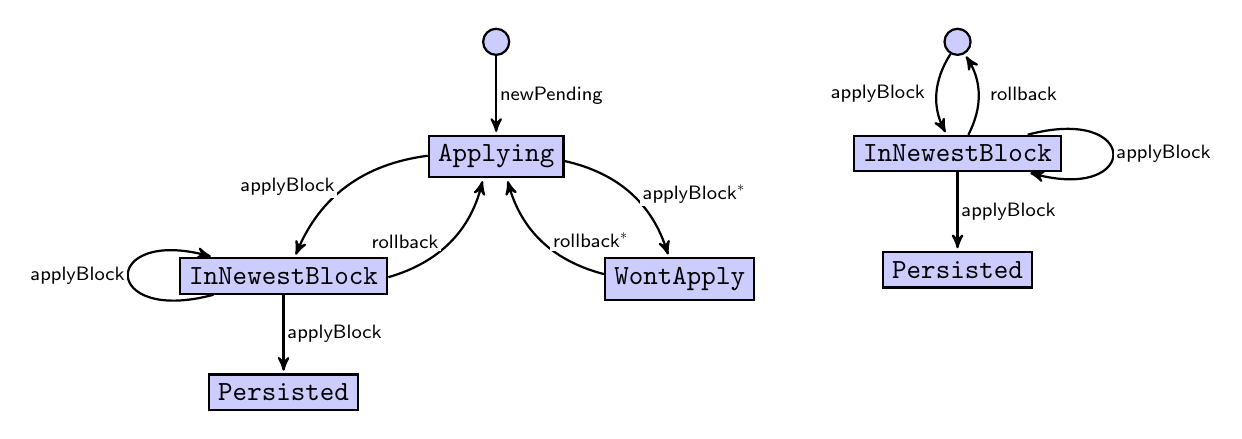
\begin{tikzpicture}[->,>=stealth',shorten >=1pt,auto,node distance=2cm,
  thick,main node/.style={rectangle,fill=blue!20,draw,minimum size=1mm}]

  \node[main node,style={circle}] (LStart) {};
  \node[main node] (LApplying)      [below=1cm of LStart] {\texttt{Applying}};
  \node[main node] (LInNewestBlock) [below left=1cm and 0.5cm of LApplying] {\texttt{InNewestBlock}};
  \node[main node] (LWontApply)     [below right=1cm and 0.5cm of LApplying] {\texttt{WontApply}};
  \node[main node] (LPersisted)     [below =1cm of LInNewestBlock] {\texttt{Persisted}};

  \path[every node/.style={font=\sffamily\scriptsize,
      fill=white,inner sep=1pt}]
    % Right-hand-side arrows rendered from top to bottom to
    % achieve proper rendering of labels over arrows.
    (LStart)
      edge node {$\mathsf{newPending}$} (LApplying)
    (LApplying)
      edge [bend right=30] node[left=1mm] {$\mathsf{applyBlock}$} (LInNewestBlock)
      edge [bend left=30]  node[right=1mm] {$\mathsf{applyBlock}^*$} (LWontApply)
    (LInNewestBlock)
      edge [loop left]     node {$\mathsf{applyBlock}$} (LInNewestBlock)
      edge [bend right=30] node[left=1mm] {$\mathsf{rollback}$} (LApplying)
      edge node {$\mathsf{applyBlock}$} (LPersisted)
    (LWontApply)
      edge [bend left=30] node[right=1mm] {$\mathsf{rollback}^*$} (LApplying)
    ;

  \node[main node,style={circle}] (RStart) [right=5.5cm of LStart] {};
  \node[main node] (RInNewestBlock) [below=1cm of RStart] {\texttt{InNewestBlock}};
  \node[main node] (RPersisted)     [below=1cm of RInNewestBlock] {\texttt{Persisted}};

  \path[every node/.style={font=\sffamily\scriptsize,
      fill=white,inner sep=1pt}]
    % Right-hand-side arrows rendered from top to bottom to
    % achieve proper rendering of labels over arrows.
    (RStart)
      edge [bend right=30] node[left=1mm] {$\mathsf{applyBlock}$} (RInNewestBlock)
    (RInNewestBlock)
      edge [loop right]     node {$\mathsf{applyBlock}$} (RInNewestBlock)
      edge [bend right=30] node[right=1mm] {$\mathsf{rollback}$} (RStart)
      edge node {$\mathsf{applyBlock}$} (RPersisted)
    ;
\end{tikzpicture}
\caption{\label{fig:transaction_state}Transaction state transitions (outgoing, \emph{left}, and incoming, \emph{right})}
\end{figure}

\section{Transaction resubmission and cancellation}

An actual implementation of the wallet needs to broadcast pending transactions
to the network, monitor when they get included in the blockchain, re-submit them
if they don't get included, and perhaps eventually decide to give up on them if
for some reason they do not get included.

The (re)submission layer can use a (priority) queue that for each time slot
records which transactions may need to be resubmitted. Each time a transaction
gets submitted in slot $n$, a resubmission gets scheduled for slot $n + l$ for
some constant $l$. When slot $n + l$ comes, the resubmission logic checks if the
transaction is still in the wallet's pending set, and if so, repeat the process.
This resubmission state can be kept separate from the core wallet state (meaning
that there is no need for some kind of consistency between the two states).

After a rollback the resubmission layer needs to figure out which transactions
have become pending again, and start the resubmission process afresh. This
could possibly be faciliated by a callback from the core wallet layer.

When the resubmission layer wants to give up on a transaction, it should
remove it from $\mathit{pending}$. From the point of view of the model
this corresponds to a new function
%
\begin{align*}
& \mathsf{cancel} :: \mathsf{Tx} \rightarrow \mathsf{Wallet} \rightarrow \mathsf{Wallet} \\
& \mathsf{cancel} ~ tx ~ (\mathit{checkpoints}, \mathit{txInfo}) = (\mathsf{map} ~ \mathsf{cancel'} ~ \mathit{checkpoints}, \mathit{txInfo}) \\
& \qquad \text{where} ~ \mathsf{cancel}' ~ (\mathit{utxo}, \mathit{pending}, \mathit{blockMeta}) = (\mathit{utxo}, \mathit{pending} \setminus \{ \mathit{tx} \}, \mathit{blockMeta})
\end{align*}
%
Note that the logic of Section~\ref{sec:transaction_status} means that such
a transaction would then be reported as $\mathtt{WontApply}$. Since we
removed the transaction from the $\mathit{pending}$ set in all checkpoints
however a rollback won't reintroduce it into $\mathit{pending}$; if the user
wants to explicitly tell the wallet to try this transaction again they will
need to call $\mathsf{newPending}$. Effectively, $\mathsf{cancel}$ becomes a
secondary way in which a transaction may go from $\texttt{Applying}$ to
$\texttt{WontApply}$ (arrow $\mathsf{applyBlock}^*$), and $\mathsf{newPending}$
a secondary way to get back from $\texttt{WontApply}$ to $\texttt{Applying}$
(arrow $\mathsf{rollback}^*$).

\paragraph{Note.} Of course, once a transaction has been broadcast, cancelling
it locally does not mean the transaction won't be included anymore. This can
only be fixed by introducing a TTL. \\

Since resubmission is time sensitive, there is not much point persisting it.
When the wallet is restarted, resubmission state can be re-initialized from
the core wallet's reported $\mathit{pending}$ set.

\section{TODO: Transaction input selection and UTxO maintenance}

\subsection{The problems}

Let us start by identifying the problems.

Selecting transaction inputs is non-trivial because of transaction fees and
because there are multiple competing goals. In a myopic view of input
selection, the distribution of coins across available inputs is assumed to be
fixed, or to be out of our control, whereas in reality we can -- at some cost
-- actively adjust the distribution.

In general the problem should be considered as optimising for certain goals
over long sequences of incoming and outgoing transactions. In this setting
the input selection and active UTxO maintenance are parts of a single policy.
To evaluate a policy we should consider scenarios, such as: steady states with
assumed distributions of values of incoming transactions and outgoing
transactions; very large payments; or emptying a wallet.

\subsection{Input selection}

The problem with fees is that the minimum fee depends on the size of the transaction
-- currently the size in bytes of the serialised representation -- but paying a
fee may require selecting more transaction inputs which increases the size.

\begin{equation}
\begin{split}
\mathsf{minfee} & \in \mathsf{Tx} \to \mathsf{Coin} \\
\mathsf{minfee} & = f \circ \mathsf{size} \circ \mathsf{serialise} \\
             & \text{where } f \text{ is some linear function}
\end{split}
\end{equation}

The actual fee for a specific transaction must be at least the minimum fee of
course. There is no fee upper bound but a `good' input selection
implementation will produce a relatively tight bound. We may wish to make that
tight bound precise such as constraining it to be within a certain factor of
the minimum fee.

\begin{equation}
\begin{split}
\mathsf{fee} ~ utxo ~ tx \geq \mathsf{minfee} ~ tx
\end{split}
\end{equation}

The fee itself is not represented explicitly in the transaction, it is a
function of the current UTxO.

\begin{equation}
\begin{split}
\mathsf{fee} & \in \mathsf{UTxO} \to \mathsf{Tx} \to \mathsf{Coin} \\
\mathsf{fee} ~ utxo ~ tx & = \mathsf{totalin} ~ utxo ~ tx - \mathsf{totalout} ~ tx
\end{split}
\end{equation}
%
\begin{equation}
\begin{split}
\mathsf{totalin} ~ utxo ~ (inputs, ~ \_) & = \mathsf{balance} ~ (inputs \restrictdom utxo) \\
                 & \text{if } inputs \subseteq \dom utxo \\
\mathsf{totalout} ~ (\_, ~ outputs) & = \sum_{(\_, c) \in outputs} c \\
\end{split}
\end{equation}

Thus fee calculation and input selection are interdependent. There are
situations where it is not immediately obvious that there is a terminating
algorithm for selecting inputs and fees optimally.

Input selection can also have multiple goals, including: minimising fees,
cryptographic security, maximising privacy and allowing high throughput. Of
course there is always the issue of acceptable time and space complexity.

The goal of minimising fees is obvious, but it is immediately plausible to see
that other goals may be in conflict since they may require picking other or
additional inputs. The goal of minimising fees highlights the fact that input
selection is not a single-shot problem. Minimising the fee of a single
transaction is not the same as minimising fees in the long term over a
sequence of transactions drawn from a distribution of transaction sizes.

The cryptographic security goal comes from the observation that once an input
at an address has been spent from, its public key is publicly known and is
arguably no longer suitable for very long term storage of funds due to the
evolution of cryptography. The standard solution with input selection is to add
a constraint that if we pick one input then we must pick all other inputs that
were output to the same address. This results in no more funds remaining at the
address (assuming an address non-reuse strategy such that there are no later
payments to that address).

The privacy goal is to make it impractical for other people observing the
transactions in the ledger to tie an identity to all the funds belonging to
that identity. In UTxO style accounting, this is typically done by an identity
holding multiple unspent transaction outputs and avoiding using them in such a
way that they can be easily associated with each other. For example, an obvious
thing to avoid is having different unspent transaction outputs at the same
address. One particular issue is the problem of the `change address' in a
transaction being easily identifiable. For example, if a very large input is
selected and a small amount is sent to one output and the remaining large
amount to another output then all observers will reasonably conclude that the
large output is the change address. Tracing transaction graphs with lots of
easy signs like this makes it much easier to

Achieving a high rate of transactions in a UTxO style ledger involves having
multiple unconfirmed transactions in-flight at once. There are hazards with
dependent in-flight transactions so to avoid them it is preferable to construct
independent transactions. For input selection this means not picking change
addresses of unconfirmed transactions. For UTxO maintenance this implies that
we must maintain a large enough supply of suitable unspent outputs. This is in
contrast to UTxO distributions that concentrate most funds in a small number of
unspent outputs.

\subsection{UTxO maintenance}

We will consider two basic use cases: exchanges and individual users. We will
see that the two use cases need policies that aim for different goals, so we
will look to design a policy for each use case.

We assume that exchanges have high rates of incoming and outgoing transactions,
large overall balances and will tend to have large UTxOs. For this use case we
are concerned with asymptotic complexity (due to the large UTxO) and have a
goal of high throughput, but we are not overly concerned with the goals of
achieving privacy or minimising fees. Exchanges tend to follow deposit policies
which are incompatible with the cryptographic security goal as described above,
so this is not a goal of the policy.

For individual users we assume a low rate of incoming and outgoing transactions
and a comparatively small UTxO. For this use case we are not too concerned with
asymptotic complexity as the UTxO is assumed to be small, nor with a goal of
high throughput. We are concerned with the privacy goal, as individual users
are able to use their wallets in a way that preserves a degree of privacy. We
are somewhat concerned with keeping fees reasonably low.

There is another goal we may wish to consider for the individual user use case:
preserving the ability to spend all or a large fraction of the total balance in
a wallet. A similar property for an exchange wallet would be maintaining the
ability to make payments up to a certain size (or fraction of the overall
balance).

\subsection{Basic specification of input selection}

Ignoring the issues of optimising for various goals, we start with the basic
problem definition and conditions on a valid solution.

Given a wallet's available UTxO and a bunch of output addresses and corresponding
amounts, pick a set of inputs and outputs to form the transaction.

\begin{equation}
\begin{split}
\mathsf{selectInputs} \in \mathsf{UTxO} \to (\mathsf{Ix} \mapsto \mathsf{TxOut})
                      \to (\powerset{\mathsf{TxId}} \times (\mathsf{Ix} \mapsto \mathsf{TxOut}))
\end{split}
\end{equation}
Obviously the inputs selected must be ones that are available in the UTxO and
the outputs requested have to be included in the outputs chosen. Additionally,
the outputs may contain change outputs and of course these must be our own
addresses so the change goes back to our wallet. And of course we must pay
transaction fees.
\begin{equation}
\begin{split}
(inputs, outputs^\prime) & = \mathsf{selectInputs} ~ utxo ~ outputs \\
outputs_{change} & = outputs^\prime \setminus outputs \\
 \Longrightarrow \quad & inputs ~ \subseteq \dom utxo \\
\wedge & ~ outputs \subseteq outputs^\prime \\
\wedge & ~ outputs_{change} \subseteq \mathsf{TxOut_{ours}} \\
\wedge & ~ \mathsf{minfee} ~ tx \leq \mathsf{fee} ~ utxo ~ (inputs, output^\prime) \leq \mathsf{minfee} ~ tx \times C\\
\end{split}
\end{equation}

\subsection{A plausible approach}

Suppose we take a UTxO relation set and arrange it into buckets based on the
coin value. We declare buckets based on powers of two, so that bucket $j$
contains inputs with coin values $c$ in the range $2^j \leq c < 2^{j+1}$. This
gives us a logarithmic number of buckets. The intuition is that if we are able
to be indifferent between unspent outputs within each bucket, then we can
select an input of any size in log time.

For basic input selection, suppose initially that there are enough unspent
outputs in each bucket, and we are trying to spend a total output (including
fees) of $2^j \leq c < 2^{j+1}$. We pick \emph{two} inputs from bucket $j$,
giving us a total output value of $2^{j+1} \leq v < 2^{j+2}$. Thus $c \leq v$.

For fees, we can derive a worst case fee formula based only on the number of
inputs and outputs. So in a typical case we can compute the worst case fee up
front and include it in the total output we are trying to spend. As a later
step we should be able to minimise the fee (computed using the actual inputs
and outputs) and shift the excess into the change address(es). It is not
essential to achieve the minimum fee, provided we can achieve a reasonable
bound in a reasonable time.

If there are not enough available inputs in the target bucket we need to have
a worst-case algorithm. This may be as follows: look for one input in higher
buckets in ascending order. If there are none, iterate over the list of buckets
from highest value to smallest, taking the total balance and size of each bucket
and accumulating a running total. And outcome is obviously possible if the total
balance (plus worst case fees) goes over the target output before the number of
inputs makes the transaction size bigger than the maximum. If both limits are
breached by adding a single bucket then it becomes necessary to sort the bucket
and do the same linear search within the bucket. In a typical case this takes
log time, but in the worst case it is n log n in the size of the offending
bucket, which in the worst case contains the entire UTxO.

In the typical case that there were enough available inputs in the target
bucket then we have not used many inputs and we should take the opportunity
to do some UTxO maintenance.

We assume we can define a policy target function which gives the ideal number
of entries in each UTxO bucket. This may be a function of the total UTxO
balance and it is likely sensible to have a parameters for lower and upper
limits on bucket size (very small inputs are not very useful, while very big
ones take up too much balance).

UTxO maintenance then consists of evaluating the function on each bucket and
seeing which buckets are above or below the ideal. The ideal function may be
real valued but of course buckets contain an integer number of entries. We
should use a threshold to avoid unnecessary movement, and at a minimum 1. Once
we know which buckets are too full or not full enough, we move entries from
buckets that are too full towards ones that are not full enough. There are of
course many ways to do this so one plausible approach is to establish some
order on how desirable each one is, and then pick in order, up to some limit
(again ultimately limited by the transaction size).

To avoid excessive UTxO rearrangement we should evaluate the use of the
threshold of how much a bucket is above or below the ideal, and/or use some
measure of how far the UTxO deviates from the ideal distribution to decide
how aggressively we should rearrange. Then this should be evaluated in
simulations over time.

\section{TODO: Persistent storage}

Threading (see prefiltering)

Batching (see rollback, definition of $\mathsf{switch}$).

\subsection{Switching to a fork}

Although $\mathsf{rollback}$ is a useful primitive operation on the wallet
state, in practice the wallet will never ever actually rollback, but rather
switch to a different fork. The disambiguation rule in the underlying blockchain
protocol (either Ouroboros or Ouroboros Praos) states that this can only happen
if that other fork is \emph{longer} than the current one.

It will therefore we useful to provide a higher-level operation that combines
rolling back with applying the blocks in the new fork:

\begin{equation}
\mathsf{switch} ~ n ~ \mathit{blocks} = \mathsf{applyBlocks} ~ \mathit{blocks} \circ \mathsf{rollbacks} ~ n
\end{equation}

where $\mathsf{rollbacks} ~ n$ calls $\mathsf{rollback}$ $n$ times, and
$\mathsf{applyBlocks}$ calls $\mathsf{applyBlock}$ for all blocks in order.
Such an operation is important because it means that the intermediate state
of the wallet during the switch is not visible to the user.

\emph{Implementation Note.} The current Cardano API does not provide something
equivalent to $\mathsf{switch}$, instead providing only hooks that correspond to
$\mathsf{applyBlocks}$ and $\mathsf{rollbacks}$. The wallet kernel however could
batch up the calls to $\mathsf{rollbacks}$, and not apply the $n$ rollbacks
until it has at least $n + m$ ($m \ge 1$) blocks to apply. This solution is not
ideal, as it is unclear what value to set $m$ to; probably the only workable
solution is to set a time bound. However, since all these $\mathsf{applyBlocks}$
will come very close together (\emph{maybe} even as a single call), in practice
this can probably work reasonably well.

\section{TODO: Lightweight wallet}

Stateless client (containing keys only) with server-side wallet state
(one server supporting multiple wallets).

\section{TODO: Wallet recovery}

Efficient wallet recovery

Also very important for the design of the light-weight wallet, where we may
spin up and tear down wallets very frequently.

\section{Next steps}

Consider confirmations / block depth.

Consider address selection, both how to do it and what information may need to
be maintained (incrementally) to do it efficiently. Partly this can be specified
and partly it needs to be simulated to establish the emergent behaviour over a
long series of transactions.

Look for other properties, e.g. wallet utxo $\subseteq$ chain utxo.

Establish storage/memory requirements.

It should be true that different instances of the `same' wallet (that do not share their pending sets) eventually end up in the same state.

Add pending tx expiry / TTL (would be needed to prove wallets end up in the same state after a finite time).

Prove properties.

\bibliographystyle{apalike}
\bibliography{references}

\end{document}
